\documentclass[12pt,%
                             a4paper,%
                             pagesize,%
                             twoside,%
                             cleardoublepage=plain,%
                             BCOR=12mm,%
                             headinclude=true,%
                             footinclude=false,%
                             DIV = 13]%
{scrartcl}
\usepackage{setspace}
\onehalfspacing
\KOMAoptions{DIV=last}

\usepackage[T1]{fontenc}
\usepackage[english]{babel}
\usepackage{ fixltx2e}
\usepackage{microtype}
\usepackage{ellipsis}

\usepackage{lmodern}

\usepackage{scrpage2}
\usepackage{amsmath}
\usepackage{amssymb}
\usepackage{graphicx}
\usepackage{multirow}
\usepackage{rotating}
\usepackage{array}
\usepackage{tabularx}
\usepackage{subfig}
\usepackage{tikz}
\usetikzlibrary{calc,shapes,arrows,decorations.pathmorphing,positioning,fit,petri,backgrounds}

\begin{document}
%%%%%%%%%%%%%%%%%%%%%%%%%%%%%%%%%%%%%%%%%%%%%%%%%%%%%%%%%%%%%%%%%%%%%%%%%%%%%%%%%
%Titelseite
%%%%%%%%%%%%%%%%%%%%
\begin{spacing}{1}
\title{MPFA-3d-Guide}
\author{}
\date{\today}
\maketitle
\end{spacing}

%%%%%%%%%%%%%%%%%%%
\section{MPFA-Guide}
\begin{figure}
\centering
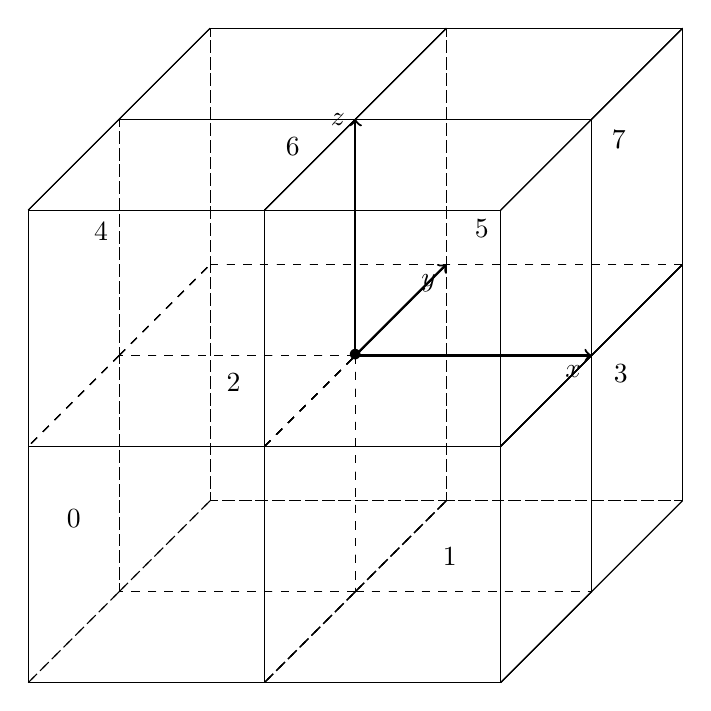
\begin{tikzpicture}[scale = 3, cm={1,0,-1,-1, (0,0)},y=-3.85mm, z = -1cm]
    \draw[thick,->,black] (0,0,0) -- (1,0,0) node[anchor=north east]{$x$};
    \draw[thick,->] (0,0,0) -- (0,1,0) node[anchor=north east]{$y$};
    \draw[thick,->] (0,0,0) -- (0,0,1) node[anchor=east]{$z$};

\node at (0,0,0) {$\bullet$};
\node at (1.2,-0.2,0) {$3$};
\node at (0.4,0,-0.85) {$1$};
\node at (0.15,1,0.15) {$5$};
\node at (1,0.3,0.8)  {$7$};
\node at (-0.4,-0.3,0){$2$};
\node at (-1,-0.2,0.6){$4$};
\node at (-1,-0.5,-0.5){$0$};
\node at (-0.65,1,0.5) {$6$};

%Cube Left Front Upper

%X-Y rectangle Z = 1
\draw[] (-1,-1,1) -- (0,-1,1);
\draw[] (0,-1,1)  -- (0,0,1);
\draw[] (0,0,1)   -- (-1,0,1);
\draw[] (-1,0,1)  -- (-1,-1,1);

%X-Z rectangle Y = -1
\draw[] (-1,-1,1) -- (-1,-1,0);
\draw[] (-1,-1,0) -- (0,-1,0);
\draw[] (0,-1,0)  -- (0,-1,1);
\draw[] (0,-1,1)  -- (-1,-1,1);

%Z-Y rectangle X = 0
\draw[] (0,-1,1) -- (0,-1,0);
\draw[dashed] (0,-1,0) -- (0,0,0);
\draw[dashed] (0,0,0)  -- (0,0,1);
\draw[]  (0,0,1) -- (0,-1,1);

%X-Y rectangle Z = 0
\draw[] (-1,-1,0) -- (0,-1,0);
\draw[dashed] (0,-1,0) -- (0,0,0);
\draw[dashed] (0,0,0)  -- (-1,0,0);
\draw[dashed] (-1,0,0) -- (-1,-1,0);

%Y-Z rectangle X = -1
\draw[] (-1,-1,0) -- (-1,-1,1);
\draw[] (-1,-1,1) -- (-1,0,1);
\draw[dashed] (-1,0,1) -- (-1,0,0);
\draw[dashed] (-1,0,0) -- (-1,-1,0);

%X-Z rectangle Y = 0
\draw[dashed] (0,0,0)  -- (-1,0,0);
\draw[dashed] (-1,0,0) -- (-1,0,1);
\draw[dashed] (0,0,0)  -- (0,0,1);
\draw[]       (0,0,1)  -- (-1,0,1);



%Cube Right Front Upper

%X-Y rectangle Z = 1
\draw[] (1,-1,1) -- (0,-1,1);
\draw[] (0,-1,1)  -- (0,0,1);
\draw[] (0,0,1)   -- (1,0,1);
\draw[] (1,0,1)  -- (1,-1,1);

%rX-Z rectangle Y = -1
\draw[] (1,-1,1) -- (1,-1,0);
\draw[] (1,-1,0) -- (0,-1,0);
\draw[] (0,-1,0)  -- (0,-1,1);
\draw[] (0,-1,1)  -- (1,-1,1);

%Y-Z rectangle X = 0
\draw[] (0,-1,1) -- (0,-1,0);
\draw[dashed] (0,-1,0) -- (0,0,0);
\draw[dashed] (0,0,0)  -- (0,0,1);
\draw[]  (0,0,1) -- (0,-1,1);

%X-Y rectangle Z = 0
\draw[] (1,-1,0) -- (0,-1,0);
\draw[dashed] (0,-1,0) -- (0,0,0);
\draw[dashed] (0,0,0)  -- (1,0,0);
\draw[] (1,0,0) -- (1,-1,0);

%Y-Z rectangle X = 1
\draw[] (1,-1,0) -- (1,-1,1);
\draw[] (1,-1,1) -- (1,0,1);
\draw[] (1,0,1) -- (1,0,0);
\draw[] (1,0,0) -- (1,-1,0);

%X-Z rectangle Y = 0
\draw[dashed] (0,0,0)  -- (1,0,0);
\draw[] (1,0,0) -- (1,0,1);
\draw[dashed] (0,0,0)  -- (0,0,1);
\draw[]       (0,0,1)  -- (1,0,1);



%Cube Right Back Upper

%X-Y rectangle Z = 1
\draw[] (1,1,1) -- (0,1,1);
\draw[] (0,1,1)  -- (0,0,1);
\draw[] (0,0,1)   -- (1,0,1);
\draw[] (1,0,1)  -- (1,1,1);

%X-Z rectangle Y = 1
\draw[] (1,1,1) -- (1,1,0);
\draw[dashed] (1,1,0) -- (0,1,0);
\draw[dashed] (0,1,0)  -- (0,1,1);
\draw[] (0,1,1)  -- (1,1,1);

%Y-Z rectangle X = 0
\draw[dashed] (0,1,1) -- (0,1,0);
\draw[dashed] (0,1,0) -- (0,0,0);
\draw[dashed] (0,0,0)  -- (0,0,1);
\draw[]  (0,0,1) -- (0,1,1);

%X-Y rectangle Z = 0
\draw[dashed] (1,1,0) -- (0,1,0);
\draw[dashed] (0,1,0) -- (0,0,0);
\draw[dashed] (0,0,0)  -- (1,0,0);
\draw[] (1,0,0) -- (1,1,0);

%Y-Z rectangle X = 1
\draw[] (1,1,0) -- (1,1,1);
\draw[] (1,1,1) -- (1,0,1);
\draw[] (1,0,1) -- (1,0,0);
\draw[] (1,0,0) -- (1,1,0);

%X-Z rectangle Y = 0
\draw[dashed] (0,0,0)  -- (1,0,0);
\draw[] (1,0,0) -- (1,0,1);
\draw[dashed] (0,0,0)  -- (0,0,1);
\draw[]       (0,0,1)  -- (1,0,1);


%Cube Left Back Upper

%X-Y rectangle Z = 1
\draw[] (-1,1,1) -- (0,1,1);
\draw[] (0,1,1)  -- (0,0,1);
\draw[] (0,0,1)   -- (-1,0,1);
\draw[] (-1,0,1)  -- (-1,1,1);

%X-Z rectangle Y = 1
\draw[dashed] (-1,1,1) -- (-1,1,0);
\draw[dashed] (-1,1,0) -- (0,1,0);
\draw[dashed] (0,1,0)  -- (0,1,1);
\draw[] (0,1,1)  -- (-1,1,1);

%Y-Z rectangle X = 0
\draw[dashed] (0,1,1) -- (0,1,0);
\draw[dashed] (0,1,0) -- (0,0,0);
\draw[dashed] (0,0,0)  -- (0,0,1);
\draw[]  (0,0,1) -- (0,1,1);

%X-Y rectangle Z = 0
\draw[dashed] (-1,1,0) -- (0,1,0);
\draw[dashed] (0,1,0) -- (0,0,0);
\draw[dashed] (0,0,0)  -- (-1,0,0);
\draw[dashed] (-1,0,0) -- (-1,1,0);

%Y-Z rectangle X = -1
\draw[dashed] (-1,1,0) -- (-1,1,1);
\draw[] (-1,1,1) -- (-1,0,1);
\draw[dashed] (-1,0,1) -- (-1,0,0);
\draw[dashed] (-1,0,0) -- (-1,1,0);

%X-Z rectangle Y = 0
\draw[dashed] (0,0,0)  -- (-1,0,0);
\draw[dashed] (-1,0,0) -- (-1,0,1);
\draw[dashed] (0,0,0)  -- (0,0,1);
\draw[]       (0,0,1)  -- (-1,0,1);


%Cube Left Front Lower

%X-Y rectangle Z = -1
\draw[] (-1,-1,-1) -- (0,-1,-1);
\draw[dashed] (0,-1,-1)  -- (0,0,-1);
\draw[dashed] (0,0,-1)   -- (-1,0,-1);
\draw[dashed] (-1,0,-1)  -- (-1,-1,-1);

%X-Z rectangle Y = -1
\draw[] (-1,-1,-1) -- (-1,-1,0);
\draw[] (-1,-1,0) -- (0,-1,0);
\draw[] (0,-1,0)  -- (0,-1,-1);
\draw[] (0,-1,-1)  -- (-1,-1,-1);

%Z-Y rectangle X = 0
\draw[] (0,-1,-1) -- (0,-1,0);
\draw[dashed] (0,-1,0) -- (0,0,0);
\draw[dashed] (0,0,0)  -- (0,0,-1);
\draw[dashed]  (0,0,-1) -- (0,-1,-1);

%X-Y rectangle Z = 0
\draw[] (-1,-1,0) -- (0,-1,0);
\draw[dashed] (0,-1,0) -- (0,0,0);
\draw[dashed] (0,0,0)  -- (-1,0,0);
\draw[dashed] (-1,0,0) -- (-1,-1,0);

%Y-Z rectangle X = -1
\draw[] (-1,-1,0) -- (-1,-1,-1);
\draw[dashed] (-1,-1,-1) -- (-1,0,-1);
\draw[dashed] (-1,0,-1) -- (-1,0,0);
\draw[dashed] (-1,0,0) -- (-1,-1,0);

%X-Z rectangle Y = 0
\draw[dashed] (0,0,0)  -- (-1,0,0);
\draw[dashed] (-1,0,0) -- (-1,0,-1);
\draw[dashed] (0,0,0)  -- (0,0,-1);
\draw[dashed]       (0,0,-1)  -- (-1,0,-1);



%Cube Right Front Lower

%X-Y rectangle Z = -1
\draw[] (1,-1,-1) -- (0,-1,-1);
\draw[dashed] (0,-1,-1)  -- (0,0,-1);
\draw[dashed] (0,0,-1)   -- (1,0,-1);
\draw[] (1,0,-1)  -- (1,-1,-1);

%rX-Z rectangle Y = -1
\draw[] (1,-1,-1) -- (1,-1,0);
\draw[] (1,-1,0) -- (0,-1,0);
\draw[] (0,-1,0)  -- (0,-1,-1);
\draw[] (0,-1,-1)  -- (1,-1,-1);

%Y-Z rectangle X = 0
\draw[] (0,-1,-1) -- (0,-1,0);
\draw[dashed] (0,-1,0) -- (0,0,0);
\draw[dashed] (0,0,0)  -- (0,0,-1);
\draw[dashed]  (0,0,-1) -- (0,-1,-1);

%X-Y rectangle Z = 0
\draw[] (1,-1,0) -- (0,-1,0);
\draw[dashed] (0,-1,0) -- (0,0,0);
\draw[dashed] (0,0,0)  -- (1,0,0);
\draw[] (1,0,0) -- (1,-1,0);

%Y-Z rectangle X = 1
\draw[] (1,-1,0) -- (1,-1,-1);
\draw[] (1,-1,-1) -- (1,0,-1);
\draw[] (1,0,-1) -- (1,0,0);
\draw[] (1,0,0) -- (1,-1,0);

%X-Z rectangle Y = 0
\draw[dashed] (0,0,0)  -- (1,0,0);
\draw[] (1,0,0) -- (1,0,-1);
\draw[dashed] (0,0,0)  -- (0,0,-1);
\draw[dashed] (0,0,-1)  -- (1,0,-1);



%Cube Right Back Lower

%X-Y rectangle Z = -1
\draw[dashed] (1,1,-1) -- (0,1,-1);
\draw[dashed] (0,1,-1)  -- (0,0,-1);
\draw[dashed] (0,0,-1)   -- (1,0,-1);
\draw[] (1,0,-1)  -- (1,1,-1);

%X-Z rectangle Y = 1
\draw[] (1,1,-1) -- (1,1,0);
\draw[dashed] (1,1,0) -- (0,1,0);
\draw[dashed] (0,1,0)  -- (0,1,-1);
\draw[dashed] (0,1,-1)  -- (1,1,-1);

%Y-Z rectangle X = 0
\draw[dashed] (0,1,1) -- (0,1,0);
\draw[dashed] (0,1,0) -- (0,0,0);
\draw[dashed] (0,0,0)  -- (0,0,-1);
\draw[dashed]  (0,0,-1) -- (0,1,-1);

%X-Y rectangle Z = 0
\draw[dashed] (1,1,0) -- (0,1,0);
\draw[dashed] (0,1,0) -- (0,0,0);
\draw[dashed] (0,0,0)  -- (1,0,0);
\draw[] (1,0,0) -- (1,1,0);

%Y-Z rectangle X = 1
\draw[] (1,1,0) -- (1,1,1);
\draw[] (1,1,1) -- (1,0,1);
\draw[] (1,0,1) -- (1,0,0);
\draw[] (1,0,0) -- (1,1,0);

%X-Z rectangle Y = 0
\draw[dashed] (0,0,0)  -- (1,0,0);
\draw[] (1,0,0) -- (1,0,-1);
\draw[dashed] (0,0,0)  -- (0,0,-1);
\draw[dashed]       (0,0,-1)  -- (1,0,-1);


%Cube Left Back Lower

%X-Y rectangle Z = -1
\draw[dashed] (-1,1,-1) -- (0,1,-1);
\draw[dashed] (0,1,-1)  -- (0,0,-1);
\draw[dashed] (0,0,-1)   -- (-1,0,-1);
\draw[dashed] (-1,0,-1)  -- (-1,1,-1);

%X-Z rectangle Y = 1
\draw[dashed] (-1,1,-1) -- (-1,1,0);
\draw[dashed] (-1,1,0) -- (0,1,0);
\draw[dashed] (0,1,0)  -- (0,1,-1);
\draw[dashed] (0,1,-1)  -- (-1,1,-1);

%Y-Z rectangle X = 0
\draw[dashed] (0,1,-1) -- (0,1,0);
\draw[dashed] (0,1,0) -- (0,0,0);
\draw[dashed] (0,0,0)  -- (0,0,-1);
\draw[dashed]  (0,0,-1) -- (0,1,-1);

%X-Y rectangle Z = 0
\draw[dashed] (-1,1,0) -- (0,1,0);
\draw[dashed] (0,1,0) -- (0,0,0);
\draw[dashed] (0,0,0)  -- (-1,0,0);
\draw[dashed] (-1,0,0) -- (-1,1,0);

%Y-Z rectangle X = -1
\draw[dashed] (-1,1,0) -- (-1,1,-1);
\draw[dashed] (-1,1,-1) -- (-1,0,-1);
\draw[dashed] (-1,0,-1) -- (-1,0,0);
\draw[dashed] (-1,0,0) -- (-1,1,0);

%X-Z rectangle Y = 0
\draw[dashed] (0,0,0)  -- (-1,0,0);
\draw[dashed] (-1,0,0) -- (-1,0,-1);
\draw[dashed] (0,0,0)  -- (0,0,-1);
\draw[dashed]       (0,0,-1)  -- (-1,0,-1);










\end{tikzpicture}

\caption{Interaction volume.}
\end{figure}

\begin{figure}
\centering
\begin{tikzpicture}[scale = 3, cm={1,0,-1,-1, (0,0)},y=-3.85mm, z = -1cm]

%Cube Left 1st Row

\node at (-0.65,-1,4) {$6$};
\node at (0,-0.5,4) {$0$};
\node at (-0.4,0,4.15) {$1$};
\node at (0.4,0,4.15) {$2$};
\node at (0.5,-1,4) {$\bullet$};

%X-Y rectangle Z = 5
\draw[] (0.5,-1,5) -- (-0.5,-1,5);
\draw[] (-0.5,-1,5)  -- (-0.5,0,5);
\draw[] (-0.5,0,5)   -- (0.5,0,5);
\draw[] (0.5,0,5)  -- (0.5,-1,5);

%rX-Z rectangle Y = -1
\draw[] (0.5,-1,5) -- (0.5,-1,4);
\draw[] (0.5,-1,4) -- (-0.5,-1,4);
\draw[] (0-0.5,-1,4)  -- (0-0.5,-1,5);
\draw[] (0-0.5,-1,5)  -- (1-0.5,-1,5);

%Y-Z rectangle X = -0.5-0.5
\draw[] (-0.5,-1,5) -- (-0.5,-1,4);
\draw[dashed] (-0.5,-1,4) -- (-0.5,0,4);
\draw[dashed] (-0.5,0,4)  -- (-0.5,0,5);
\draw[]  (0-0.5,0,5) -- (0-0.5,-1,5);

%X-Y rectangle Z = 4
\draw[] (1-0.5,-1,4) -- (0-0.5,-1,4);
\draw[dashed] (0-0.5,-1,4) -- (0-0.5,0,4);
\draw[dashed] (0-0.5,0,4)  -- (1-0.5,0,4);
\draw[] (1-0.5,0,4) -- (1-0.5,-1,4);

%Y-Z rectangle X = 1-0.5
\draw[] (1-0.5,-1,4) -- (1-0.5,-1,5);
\draw[] (1-0.5,-1,5) -- (1-0.5,0,5);
\draw[] (1-0.5,0,5) -- (1-0.5,0,4);
\draw[] (1-0.5,0,4) -- (1-0.5,-1,4);

%X-Z rectangle Y = 0
\draw[dashed] (0-0.5,0,4)  -- (1-0.5,0,4);
\draw[] (1-0.5,0,5) -- (1-0.5,0,5);
\draw[dashed] (0-0.5,0,5)  -- (0-0.5,0,5);
\draw[]       (0-0.5,0,5)  -- (1-0.5,0,5);


%Cube Left 2nd Row

\node at (-1.65,-1,2.5) {$4$};
\node at (-1,-0.5,2.5) {$0$};
\node at (-0.5,-0.5,3) {$1$};
\node at (-1,0,3) {$2$};
\node at (-0.5,0,2.5) {$\bullet$};

%X-Y rectangle Z = 3,5
\draw[] (1-1.5,-1,3.5) -- (0-1.5,-1,3.5);
\draw[] (0-1.5,-1,3.5)  -- (0-1.5,0,3.5);
\draw[] (0-1.5,0,3.5)   -- (1-1.5,0,3.5);
\draw[] (1-1.5,0,3.5)  -- (1-1.5,-1,3.5);

%rX-Z rectangle Y = -1
\draw[] (1-1.5,-1,3.5) -- (1-1.5,-1,2.5);
\draw[] (1-1.5,-1,2.5) -- (0-1.5,-1,2.5);
\draw[] (0-1.5,-1,2.5)  -- (0-1.5,-1,3.5);
\draw[] (0-1.5,-1,3.5)  -- (1-1.5,-1,3.5);

%Y-Z rectangle X = 0-1.5
\draw[] (0-1.5,-1,3.5) -- (0-1.5,-1,2.5);
\draw[dashed] (0-1.5,-1,2.5) -- (0-1.5,0,2.5);
\draw[dashed] (0-1.5,0,2.5)  -- (0-1.5,0,3.5);
\draw[]  (0-1.5,0,3.5) -- (0-1.5,-1,3.5);

%X-Y rectangle Z = 2.5
\draw[] (1-1.5,-1,2.5) -- (0-1.5,-1,2.5);
\draw[dashed] (0-1.5,-1,2.5) -- (0-1.5,0,2.5);
\draw[dashed] (0-1.5,0,2.5)  -- (1-1.5,0,2.5);
\draw[] (1-1.5,0,2.5) -- (1-1.5,-1,2.5);

%Y-Z rectangle X = 1-1.5
\draw[] (1-1.5,-1,2.5) -- (1-1.5,-1,3.5);
\draw[] (1-1.5,-1,3.5) -- (1-1.5,0,3.5);
\draw[] (1-1.5,0,3.5) -- (1-1.5,0,2.5);
\draw[] (1-1.5,0,2.5) -- (1-1.5,-1,2.5);

%X-Z rectangle Y = 0
\draw[dashed] (0-1.5,0,2.5)  -- (1-1.5,0,2.5);
\draw[] (1-1.5,0,3.5) -- (1-1.5,0,3.5);
\draw[dashed] (0-1.5,0,3.5)  -- (0-1.5,0,3.5);
\draw[]       (0-1.5,0,3.5)  -- (1-1.5,0,3.5);


%Cube Left 3rd Row

\node at (-0.65,-1,1) {$2$};
\node at (-0.4,0,1.1) {$0$};
\node at (0.5,-0.5,1.5) {$1$};
\node at (0,-0.5,2) {$2$};
\node at (0.5,-1,2) {$\bullet$};

%X-Y rectangle Z = 2
\draw[] (1-0.5,-1,2) -- (0-0.5,-1,2);
\draw[] (0-0.5,-1,2)  -- (0-0.5,0,2);
\draw[] (0-0.5,0,2)   -- (1-0.5,0,2);
\draw[] (1-0.5,0,2)  -- (1-0.5,-1,2);

%rX-Z rectangle Y = -1
\draw[] (1-0.5,-1,2) -- (1-0.5,-1,1);
\draw[] (1-0.5,-1,1) -- (0-0.5,-1,1);
\draw[] (0-0.5,-1,1)  -- (0-0.5,-1,2);
\draw[] (0-0.5,-1,2)  -- (1-0.5,-1,2);

%Y-Z rectangle X = 0-0.5
\draw[] (0-0.5,-1,2) -- (0-0.5,-1,1);
\draw[dashed] (0-0.5,-1,1) -- (0-0.5,0,1);
\draw[dashed] (0-0.5,0,1)  -- (0-0.5,0,2);
\draw[]  (0-0.5,0,2) -- (0-0.5,-1,2);

%X-Y rectangle Z = 1
\draw[] (1-0.5,-1,1) -- (0-0.5,-1,1);
\draw[dashed] (0-0.5,-1,1) -- (0-0.5,0,1);
\draw[dashed] (0-0.5,0,1)  -- (1-0.5,0,1);
\draw[] (1-0.5,0,1) -- (1-0.5,-1,1);

%Y-Z rectangle X = 1-0.5
\draw[] (1-0.5,-1,1) -- (1-0.5,-1,2);
\draw[] (1-0.5,-1,2) -- (1-0.5,0,2);
\draw[] (1-0.5,0,2) -- (1-0.5,0,1);
\draw[] (1-0.5,0,1) -- (1-0.5,-1,1);

%X-Z rectangle Y = 0
\draw[dashed] (0-0.5,0,1)  -- (1-0.5,0,1);
\draw[] (1-0.5,0,2) -- (1-0.5,0,2);
\draw[dashed] (0-0.5,0,2)  -- (0-0.5,0,2);
\draw[]       (0-0.5,0,2)  -- (1-0.5,0,2);


%Cube Left 4th Row

\node at (-1.65,-1,-0.5) {$0$};
\node at (-0.5,-0.5,0) {$0$};
\node at (-1,0,0) {$1$};
\node at (-1,-0.5,0.5) {$2$};
\node at (-0.5,0,0.5) {$\bullet$};

%X-Y rectangle Z = 0,5
\draw[] (1-1.5,-1,0.5) -- (0-1.5,-1,0.5);
\draw[] (0-1.5,-1,0.5)  -- (0-1.5,0,0.5);
\draw[] (0-1.5,0,0.5)   -- (1-1.5,0,0.5);
\draw[] (1-1.5,0,0.5)  -- (1-1.5,-1,0.5);

%rX-Z rectangle Y = -1
\draw[] (1-1.5,-1,0.5) -- (1-1.5,-1,-0.5);
\draw[] (1-1.5,-1,-0.5) -- (0-1.5,-1,-0.5);
\draw[] (0-1.5,-1,-0.5)  -- (0-1.5,-1,0.5);
\draw[] (0-1.5,-1,0.5)  -- (1-1.5,-1,0.5);

%Y-Z rectangle X = 0-1.5
\draw[] (0-1.5,-1,0.5) -- (0-1.5,-1,-0.5);
\draw[dashed] (0-1.5,-1,-0.5) -- (0-1.5,0,-0.5);
\draw[dashed] (0-1.5,0,-0.5)  -- (0-1.5,0,0.5);
\draw[]  (0-1.5,0,0.5) -- (0-1.5,-1,0.5);

%X-Y rectangle Z = -0.5
\draw[] (1-1.5,-1,-0.5) -- (0-1.5,-1,-0.5);
\draw[dashed] (0-1.5,-1,-0.5) -- (0-1.5,0,-0.5);
\draw[dashed] (0-1.5,0,-0.5)  -- (1-1.5,0,-0.5);
\draw[] (1-1.5,0,-0.5) -- (1-1.5,-1,-0.5);

%Y-Z rectangle X = 1-1.5
\draw[] (1-1.5,-1,-0.5) -- (1-1.5,-1,0.5);
\draw[] (1-1.5,-1,0.5) -- (1-1.5,0,0.5);
\draw[] (1-1.5,0,0.5) -- (1-1.5,0,-0.5);
\draw[] (1-1.5,0,-0.5) -- (1-1.5,-1,-0.5);

%X-Z rectangle Y = 0
\draw[dashed] (0-1.5,0,-0.5)  -- (1-1.5,0,-0.5);
\draw[] (1-1.5,0,0.5) -- (1-1.5,0,0.5);
\draw[dashed] (0-1.5,0,0.5)  -- (0-1.5,0,0.5);
\draw[]       (0-1.5,0,0.5)  -- (1-1.5,0,0.5);


%Cube Right 1st Row

\node at (1.5,-0.5,4) {$0$};
\node at (1,-0.5,4.5) {$1$};
\node at (1.5,0,4.5)  {$2$};
\node at (0.85,-1,4)  {$7$};
\node at (1,-1,4)     {$\bullet$};

%X-Y rectangle Z = 5
\draw[] (2,-1,5) -- (1,-1,5);
\draw[] (1,-1,5)  -- (1,0,5);
\draw[] (1,0,5)   -- (2,0,5);
\draw[] (2,0,5)  -- (2,-1,5);

%rX-Z rectangle Y = -1
\draw[] (2,-1,5) -- (2,-1,4);
\draw[] (2,-1,4) -- (1,-1,4);
\draw[] (0+1,-1,4)  -- (0+1,-1,5);
\draw[] (0+1,-1,5)  -- (1+1,-1,5);

%Y-Z rectangle X = 1
\draw[] (1,-1,5) -- (1,-1,4);
\draw[dashed] (1,-1,4) -- (1,0,4);
\draw[dashed] (1,0,4)  -- (1,0,5);
\draw[]  (0+1,0,5) -- (0+1,-1,5);

%X-Y rectangle Z = 4
\draw[] (1+1,-1,4) -- (0+1,-1,4);
\draw[dashed] (0+1,-1,4) -- (0+1,0,4);
\draw[dashed] (0+1,0,4)  -- (1+1,0,4);
\draw[] (1+1,0,4) -- (1+1,-1,4);

%Y-Z rectangle X = 1+1
\draw[] (1+1,-1,4) -- (1+1,-1,5);
\draw[] (1+1,-1,5) -- (1+1,0,5);
\draw[] (1+1,0,5) -- (1+1,0,4);
\draw[] (1+1,0,4) -- (1+1,-1,4);

%X-Z rectangle Y = 0
\draw[dashed] (0+1,0,4)  -- (1+1,0,4);
\draw[] (1+1,0,5) -- (1+1,0,5);
\draw[dashed] (0+1,0,5)  -- (0+1,0,5);
\draw[]       (0+1,0,5)  -- (1+1,0,5);


%Cube Right 2nd Row

\node at (0.5,-0.5,2.5) {$0$};
\node at (0,-0.5,3)     {$2$};
\node at (0.5,0,3)      {$1$};
\node at (-0.15,-1,2.5) {$5$};
\node at (0,0,2.5)     {$\bullet$};

%X-Y rectangle Z = 3,5
\draw[] (1,-1,3.5) -- (0,-1,3.5);
\draw[] (0,-1,3.5)  -- (0,0,3.5);
\draw[] (0,0,3.5)   -- (1,0,3.5);
\draw[] (1,0,3.5)  -- (1,-1,3.5);

%rX-Z rectangle Y = -1
\draw[] (1,-1,3.5) -- (1,-1,2.5);
\draw[] (1,-1,2.5) -- (0,-1,2.5);
\draw[] (0,-1,2.5)  -- (0,-1,3.5);
\draw[] (0,-1,3.5)  -- (1,-1,3.5);

%Y-Z rectangle X = 0
\draw[] (0,-1,3.5) -- (0,-1,2.5);
\draw[dashed] (0,-1,2.5) -- (0,0,2.5);
\draw[dashed] (0,0,2.5)  -- (0,0,3.5);
\draw[]  (0,0,3.5) -- (0,-1,3.5);

%X-Y rectangle Z = 2.5
\draw[] (1,-1,2.5) -- (0,-1,2.5);
\draw[dashed] (0,-1,2.5) -- (0,0,2.5);
\draw[dashed] (0,0,2.5)  -- (1,0,2.5);
\draw[] (1,0,2.5) -- (1,-1,2.5);

%Y-Z rectangle X = 1
\draw[] (1,-1,2.5) -- (1,-1,3.5);
\draw[] (1,-1,3.5) -- (1,0,3.5);
\draw[] (1,0,3.5) -- (1,0,2.5);
\draw[] (1,0,2.5) -- (1,-1,2.5);

%X-Z rectangle Y = 0
\draw[dashed] (0,0,2.5)  -- (1,0,2.5);
\draw[] (1,0,3.5) -- (1,0,3.5);
\draw[dashed] (0,0,3.5)  -- (0,0,3.5);
\draw[]       (0,0,3.5)  -- (1,0,3.5);


%Cube Right 3rd Row

\node at (1.5,-0.5,2)  {$2$};
\node at (1.5,0,1.5)   {$1$};
\node at (1,-0.5,1.5)  {$0$};
\node at (0.85,-1,1)   {$3$};
\node at (1,-1,2)      {$\bullet$};

%X-Y rectangle Z = 2
\draw[] (1+1,-1,2) -- (0+1,-1,2);
\draw[] (0+1,-1,2)  -- (0+1,0,2);
\draw[] (0+1,0,2)   -- (1+1,0,2);
\draw[] (1+1,0,2)  -- (1+1,-1,2);

%rX-Z rectangle Y = -1
\draw[] (1+1,-1,2) -- (1+1,-1,1);
\draw[] (1+1,-1,1) -- (0+1,-1,1);
\draw[] (0+1,-1,1)  -- (0+1,-1,2);
\draw[] (0+1,-1,2)  -- (1+1,-1,2);

%Y-Z rectangle X = 1
\draw[] (0+1,-1,2) -- (0+1,-1,1);
\draw[dashed] (0+1,-1,1) -- (0+1,0,1);
\draw[dashed] (0+1,0,1)  -- (0+1,0,2);
\draw[]  (0+1,0,2) -- (0+1,-1,2);

%X-Y rectangle Z = 1
\draw[] (1+1,-1,1) -- (0+1,-1,1);
\draw[dashed] (0+1,-1,1) -- (0+1,0,1);
\draw[dashed] (0+1,0,1)  -- (1+1,0,1);
\draw[] (1+1,0,1) -- (1+1,-1,1);

%Y-Z rectangle X = 2
\draw[] (1+1,-1,1) -- (1+1,-1,2);
\draw[] (1+1,-1,2) -- (1+1,0,2);
\draw[] (1+1,0,2) -- (1+1,0,1);
\draw[] (1+1,0,1) -- (1+1,-1,1);

%X-Z rectangle Y = 0
\draw[dashed] (0+1,0,1)  -- (1+1,0,1);
\draw[] (1+1,0,2) -- (1+1,0,2);
\draw[dashed] (0+1,0,2)  -- (0+1,0,2);
\draw[]       (0+1,0,2)  -- (1+1,0,2);


%Cube Right 4th Row

\node at (0.5,-0.5,0.5)  {$2$};
\node at (0.5,-0.5,0)    {$0$};
\node at (0,-0.5,0)      {$1$};
\node at (-0.15,-1,-0.5) {$1$};
\node at (0,0,0.5)       {$\bullet$};

%X-Y rectangle Z = 0,5
\draw[] (1,-1,0.5) -- (0,-1,0.5);
\draw[] (0,-1,0.5)  -- (0,0,0.5);
\draw[] (0,0,0.5)   -- (1,0,0.5);
\draw[] (1,0,0.5)  -- (1,-1,0.5);

%rX-Z rectangle Y = -1
\draw[] (1,-1,0.5) -- (1,-1,-0.5);
\draw[] (1,-1,-0.5) -- (0,-1,-0.5);
\draw[] (0,-1,-0.5)  -- (0,-1,0.5);
\draw[] (0,-1,0.5)  -- (1,-1,0.5);

%Y-Z rectangle X = 0
\draw[] (0,-1,0.5) -- (0,-1,-0.5);
\draw[dashed] (0,-1,-0.5) -- (0,0,-0.5);
\draw[dashed] (0,0,-0.5)  -- (0,0,0.5);
\draw[]  (0,0,0.5) -- (0,-1,0.5);

%X-Y rectangle Z = -0.5
\draw[] (1,-1,-0.5) -- (0,-1,-0.5);
\draw[dashed] (0,-1,-0.5) -- (0,0,-0.5);
\draw[dashed] (0,0,-0.5)  -- (1,0,-0.5);
\draw[] (1,0,-0.5) -- (1,-1,-0.5);

%Y-Z rectangle X = 1
\draw[] (1,-1,-0.5) -- (1,-1,0.5);
\draw[] (1,-1,0.5) -- (1,0,0.5);
\draw[] (1,0,0.5) -- (1,0,-0.5);
\draw[] (1,0,-0.5) -- (1,-1,-0.5);

%X-Z rectangle Y = 0
\draw[dashed] (0,0,-0.5)  -- (1,0,-0.5);
\draw[] (1,0,0.5) -- (1,0,0.5);
\draw[dashed] (0,0,0.5)  -- (0,0,0.5);
\draw[]       (0,0,0.5)  -- (1,0,0.5);




\end{tikzpicture}
\caption{SubVolumeFaceIdxInInside.}
\end{figure}

\begin{figure}
\centering
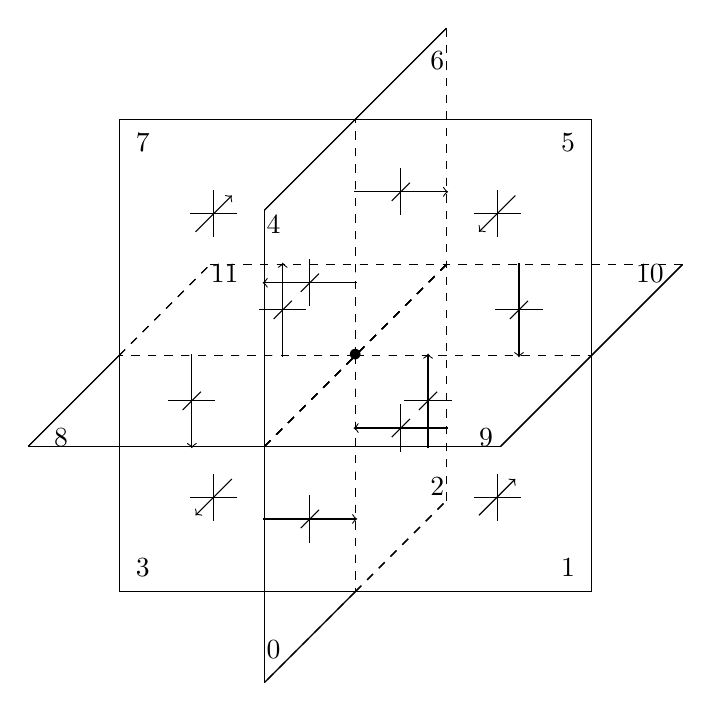
\begin{tikzpicture}[scale = 3, cm={1,0,-1,-1, (0,0)},y=-3.85mm, z = -1cm]


\node at (0,0,0) {$\bullet$};
\node at (0.9,0,-0.9)   {$1$};
\node at (0,0.9,-0.9)   {$2$};
\node at (-0.9,0,-0.9)  {$3$};
\node at (0,-0.9,-0.9)  {$0$};
\node at (0.9,-0.9,0)   {$9$};
\node at (-0.9,-0.9,0)  {$8$};
\node at (-0.9,0.9,0)   {$11$};
\node at (0.9,0.9,0)    {$10$};
\node at (-0.9,0,0.9)   {$7$};
\node at (0.9,0,0.9)    {$5$};
\node at (0,-0.9,0.9)   {$4$};
\node at (0,0.9,0.9)    {$6$};

%Cube Left Front Upper


%Z-Y rectangle X = 0
\draw[] (0,-1,1) -- (0,-1,0);
\draw[dashed] (0,-1,0) -- (0,0,0);
\draw[dashed] (0,0,0)  -- (0,0,1);
\draw[]  (0,0,1) -- (0,-1,1);

%X-Y rectangle Z = 0
\draw[] (-1,-1,0) -- (0,-1,0);
\draw[dashed] (0,-1,0) -- (0,0,0);
\draw[dashed] (0,0,0)  -- (-1,0,0);
\draw[] (-1,0,0) -- (-1,-1,0);

%X-Z rectangle Y = 0
\draw[dashed] (0,0,0)  -- (-1,0,0);
\draw[] (-1,0,0) -- (-1,0,1);
\draw[dashed] (0,0,0)  -- (0,0,1);
\draw[]       (0,0,1)  -- (-1,0,1);



%Cube Right Front Upper

%Y-Z rectangle X = 0
\draw[] (0,-1,1) -- (0,-1,0);
\draw[dashed] (0,-1,0) -- (0,0,0);
\draw[dashed] (0,0,0)  -- (0,0,1);
\draw[]  (0,0,1) -- (0,-1,1);

%X-Y rectangle Z = 0
\draw[] (1,-1,0) -- (0,-1,0);
\draw[dashed] (0,-1,0) -- (0,0,0);
\draw[dashed] (0,0,0)  -- (1,0,0);
\draw[] (1,0,0) -- (1,-1,0);

%X-Z rectangle Y = 0
\draw[dashed] (0,0,0)  -- (1,0,0);
\draw[] (1,0,0) -- (1,0,1);
\draw[dashed] (0,0,0)  -- (0,0,1);
\draw[]       (0,0,1)  -- (1,0,1);



%Cube Right Back Upper

%Y-Z rectangle X = 0
\draw[dashed] (0,1,1) -- (0,1,0);
\draw[dashed] (0,1,0) -- (0,0,0);
\draw[dashed] (0,0,0)  -- (0,0,1);
\draw[]  (0,0,1) -- (0,1,1);

%X-Y rectangle Z = 0
\draw[dashed] (1,1,0) -- (0,1,0);
\draw[dashed] (0,1,0) -- (0,0,0);
\draw[dashed] (0,0,0)  -- (1,0,0);
\draw[] (1,0,0) -- (1,1,0);

%X-Z rectangle Y = 0
\draw[dashed] (0,0,0)  -- (1,0,0);
\draw[] (1,0,0) -- (1,0,1);
\draw[dashed] (0,0,0)  -- (0,0,1);
\draw[]       (0,0,1)  -- (1,0,1);


%Cube Left Back Upper

%Y-Z rectangle X = 0
\draw[dashed] (0,1,1) -- (0,1,0);
\draw[dashed] (0,1,0) -- (0,0,0);
\draw[dashed] (0,0,0)  -- (0,0,1);
\draw[]  (0,0,1) -- (0,1,1);

%X-Y rectangle Z = 0
\draw[dashed] (-1,1,0) -- (0,1,0);
\draw[dashed] (0,1,0) -- (0,0,0);
\draw[dashed] (0,0,0)  -- (-1,0,0);
\draw[dashed] (-1,0,0) -- (-1,1,0);

%X-Z rectangle Y = 0
\draw[dashed] (0,0,0)  -- (-1,0,0);
\draw[dashed] (-1,0,0) -- (-1,0,1);
\draw[dashed] (0,0,0)  -- (0,0,1);
\draw[]       (0,0,1)  -- (-1,0,1);


%Cube Left Front Lower

%Z-Y rectangle X = 0
\draw[] (0,-1,-1) -- (0,-1,0);
\draw[dashed] (0,-1,0) -- (0,0,0);
\draw[dashed] (0,0,0)  -- (0,0,-1);
\draw[]  (0,0,-1) -- (0,-1,-1);

%X-Y rectangle Z = 0
\draw[] (-1,-1,0) -- (0,-1,0);
\draw[dashed] (0,-1,0) -- (0,0,0);
\draw[dashed] (0,0,0)  -- (-1,0,0);
\draw[] (-1,0,0) -- (-1,-1,0);

%X-Z rectangle Y = 0
\draw[dashed] (0,0,0)  -- (-1,0,0);
\draw[] (-1,0,0) -- (-1,0,-1);
\draw[dashed] (0,0,0)  -- (0,0,-1);
\draw[] (0,0,-1)  -- (-1,0,-1);



%Cube Right Front Lower

%Y-Z rectangle X = 0
\draw[] (0,-1,-1) -- (0,-1,0);
\draw[dashed] (0,-1,0) -- (0,0,0);
\draw[dashed] (0,0,0)  -- (0,0,-1);
\draw[dashed]  (0,0,-1) -- (0,-1,-1);

%X-Y rectangle Z = 0
\draw[] (1,-1,0) -- (0,-1,0);
\draw[dashed] (0,-1,0) -- (0,0,0);
\draw[dashed] (0,0,0)  -- (1,0,0);
\draw[] (1,0,0) -- (1,-1,0);

%X-Z rectangle Y = 0
\draw[dashed] (0,0,0)  -- (1,0,0);
\draw[] (1,0,0) -- (1,0,-1);
\draw[dashed] (0,0,0)  -- (0,0,-1);
\draw[] (0,0,-1)  -- (1,0,-1);



%Cube Right Back Lower

%Y-Z rectangle X = 0
\draw[dashed] (0,1,1) -- (0,1,0);
\draw[dashed] (0,1,0) -- (0,0,0);
\draw[dashed] (0,0,0)  -- (0,0,-1);
\draw[dashed]  (0,0,-1) -- (0,1,-1);

%X-Y rectangle Z = 0
\draw[dashed] (1,1,0) -- (0,1,0);
\draw[dashed] (0,1,0) -- (0,0,0);
\draw[dashed] (0,0,0)  -- (1,0,0);
\draw[] (1,0,0) -- (1,1,0);

%X-Z rectangle Y = 0
\draw[dashed] (0,0,0)  -- (1,0,0);
\draw[] (1,0,0) -- (1,0,-1);
\draw[dashed] (0,0,0)  -- (0,0,-1);
\draw[dashed]       (0,0,-1)  -- (1,0,-1);


%Cube Left Back Lower

%Y-Z rectangle X = 0
\draw[dashed] (0,1,-1) -- (0,1,0);
\draw[dashed] (0,1,0) -- (0,0,0);
\draw[dashed] (0,0,0)  -- (0,0,-1);
\draw[dashed]  (0,0,-1) -- (0,1,-1);

%X-Y rectangle Z = 0
\draw[dashed] (-1,1,0) -- (0,1,0);
\draw[dashed] (0,1,0) -- (0,0,0);
\draw[dashed] (0,0,0)  -- (-1,0,0);
\draw[dashed] (-1,0,0) -- (-1,1,0);

%X-Z rectangle Y = 0
\draw[dashed] (0,0,0)  -- (-1,0,0);
\draw[dashed] (-1,0,0) -- (-1,0,-1);
\draw[dashed] (0,0,0)  -- (0,0,-1);
\draw[dashed]       (0,0,-1)  -- (-1,0,-1);


%Arrows
\draw[->] (0.6,-0.2,-0.6) -- (0.6,0.2,-0.6);
\draw[]   (0.5,0,-0.6)    -- (0.7,0,-0.6);
\draw[]   (0.6,0,-0.5)    -- (0.6,0,-0.7);

\draw[<-] (0.2,-0.5,-0.5) -- (-0.2,-0.5,-0.5);
\draw[]   (0,-0.6,-0.5)   -- (0,-0.4,-0.5);
\draw[]   (0,-0.5,-0.6)   -- (0,-0.5,-0.4);

\draw[->] (0.2,0.5,-0.5) -- (-0.2,0.5,-0.5);
\draw[]   (0,0.6,-0.5)   -- (0,0.4,-0.5);
\draw[]   (0,0.5,-0.6)   -- (0,0.5,-0.4);

\draw[<-] (0.6,-0.2,0.6) -- (0.6,0.2,0.6);
\draw[]   (0.5,0,0.6)    -- (0.7,0,0.6);
\draw[]   (0.6,0,0.5)    -- (0.6,0,0.7);

\draw[->] (-0.6,-0.2,0.6) -- (-0.6,0.2,0.6);
\draw[]   (-0.5,0,0.6)    -- (-0.7,0,0.6);
\draw[]   (-0.6,0,0.5)    -- (-0.6,0,0.7);

\draw[<-] (-0.6,-0.2,-0.6) -- (-0.6,0.2,-0.6);
\draw[]   (-0.5,0,-0.6)    -- (-0.7,0,-0.6);
\draw[]   (-0.6,0,-0.5)    -- (-0.6,0,-0.7);

\draw[->] (0.2,-0.5,0.5) -- (-0.2,-0.5,0.5);
\draw[]   (0,-0.6,0.5)   -- (0,-0.4,0.5);
\draw[]   (0,-0.5,0.6)   -- (0,-0.5,0.4);

\draw[<-] (0.2,0.5,0.5) -- (-0.2,0.5,0.5);
\draw[]   (0,0.6,0.5)   -- (0,0.4,0.5);
\draw[]   (0,0.5,0.6)   -- (0,0.5,0.4);

\draw[->] (0.5,-0.5,-0.2) -- (0.5,-0.5,0.2);
\draw[]   (0.6,-0.5,0)    -- (0.4,-0.5,0);
\draw[]   (0.5,-0.4,0)    -- (0.5,-0.6,0);

\draw[<-] (-0.5,-0.5,-0.2) -- (-0.5,-0.5,0.2);
\draw[]   (-0.6,-0.5,0)    -- (-0.4,-0.5,0);
\draw[]   (-0.5,-0.4,0)    -- (-0.5,-0.6,0);

\draw[->] (-0.5,0.5,-0.2) -- (-0.5,0.5,0.2);
\draw[]   (-0.6,0.5,0)    -- (-0.4,0.5,0);
\draw[]   (-0.5,0.4,0)    -- (-0.5,0.6,0);

\draw[<-] (0.5,0.5,-0.2) -- (0.5,0.5,0.2);
\draw[]   (0.6,0.5,0)    -- (0.4,0.5,0);
\draw[]   (0.5,0.4,0)    -- (0.5,0.6,0);


\end{tikzpicture}

\caption{SubVolumeFace.}
\end{figure}

\begin{figure}
\centering
\begin{tikzpicture}[scale = 3, cm={1,0,-1,-1, (0,0)},y=-3.85mm, z = -1cm]

%Cube Left 1st Row

\node at (-0.65,-1,4) {$6$};
\node at (0,-1,3.95) {$0$};
\node at (0,-1,4.05) {$1$};
\node at (0.55,-1,4.5) {$1$};
\node at (0.45,-1,4.5) {$0$};
\node at (0.5,-0.5,3.95) {$1$};
\node at (0.5,-0.5,4.05) {$0$};
\node at (0.5,-1,4) {$\bullet$};

%X-Y rectangle Z = 5
\draw[] (0.5,-1,5) -- (-0.5,-1,5);
\draw[] (-0.5,-1,5)  -- (-0.5,0,5);
\draw[] (-0.5,0,5)   -- (0.5,0,5);
\draw[] (0.5,0,5)  -- (0.5,-1,5);

%rX-Z rectangle Y = -1
\draw[] (0.5,-1,5) -- (0.5,-1,4);
\draw[] (0.5,-1,4) -- (-0.5,-1,4);
\draw[] (0-0.5,-1,4)  -- (0-0.5,-1,5);
\draw[] (0-0.5,-1,5)  -- (1-0.5,-1,5);

%Y-Z rectangle X = -0.5-0.5
\draw[] (-0.5,-1,5) -- (-0.5,-1,4);
\draw[dashed] (-0.5,-1,4) -- (-0.5,0,4);
\draw[dashed] (-0.5,0,4)  -- (-0.5,0,5);
\draw[]  (0-0.5,0,5) -- (0-0.5,-1,5);

%X-Y rectangle Z = 4
\draw[] (1-0.5,-1,4) -- (0-0.5,-1,4);
\draw[dashed] (0-0.5,-1,4) -- (0-0.5,0,4);
\draw[dashed] (0-0.5,0,4)  -- (1-0.5,0,4);
\draw[] (1-0.5,0,4) -- (1-0.5,-1,4);

%Y-Z rectangle X = 1-0.5
\draw[] (1-0.5,-1,4) -- (1-0.5,-1,5);
\draw[] (1-0.5,-1,5) -- (1-0.5,0,5);
\draw[] (1-0.5,0,5) -- (1-0.5,0,4);
\draw[] (1-0.5,0,4) -- (1-0.5,-1,4);

%X-Z rectangle Y = 0
\draw[dashed] (0-0.5,0,4)  -- (1-0.5,0,4);
\draw[] (1-0.5,0,5) -- (1-0.5,0,5);
\draw[dashed] (0-0.5,0,5)  -- (0-0.5,0,5);
\draw[]       (0-0.5,0,5)  -- (1-0.5,0,5);


%Cube Left 2nd Row

\node at (-1.65,-1,2.5) {$4$};
\node at (-0.5,-0.5,2.45) {$1$};
\node at (-0.5,-0.5,2.55) {$0$};
\node at (-0.55,0,3) {$1$};
\node at (-0.45,0,3) {$0$};
\node at (-1,0,2.55) {$0$};
\node at (-1,0,2.45) {$1$};
\node at (-0.5,0,2.5) {$\bullet$};

%X-Y rectangle Z = 3,5
\draw[] (1-1.5,-1,3.5) -- (0-1.5,-1,3.5);
\draw[] (0-1.5,-1,3.5)  -- (0-1.5,0,3.5);
\draw[] (0-1.5,0,3.5)   -- (1-1.5,0,3.5);
\draw[] (1-1.5,0,3.5)  -- (1-1.5,-1,3.5);

%rX-Z rectangle Y = -1
\draw[] (1-1.5,-1,3.5) -- (1-1.5,-1,2.5);
\draw[] (1-1.5,-1,2.5) -- (0-1.5,-1,2.5);
\draw[] (0-1.5,-1,2.5)  -- (0-1.5,-1,3.5);
\draw[] (0-1.5,-1,3.5)  -- (1-1.5,-1,3.5);

%Y-Z rectangle X = 0-1.5
\draw[] (0-1.5,-1,3.5) -- (0-1.5,-1,2.5);
\draw[dashed] (0-1.5,-1,2.5) -- (0-1.5,0,2.5);
\draw[dashed] (0-1.5,0,2.5)  -- (0-1.5,0,3.5);
\draw[]  (0-1.5,0,3.5) -- (0-1.5,-1,3.5);

%X-Y rectangle Z = 2.5
\draw[] (1-1.5,-1,2.5) -- (0-1.5,-1,2.5);
\draw[dashed] (0-1.5,-1,2.5) -- (0-1.5,0,2.5);
\draw[dashed] (0-1.5,0,2.5)  -- (1-1.5,0,2.5);
\draw[] (1-1.5,0,2.5) -- (1-1.5,-1,2.5);

%Y-Z rectangle X = 1-1.5
\draw[] (1-1.5,-1,2.5) -- (1-1.5,-1,3.5);
\draw[] (1-1.5,-1,3.5) -- (1-1.5,0,3.5);
\draw[] (1-1.5,0,3.5) -- (1-1.5,0,2.5);
\draw[] (1-1.5,0,2.5) -- (1-1.5,-1,2.5);

%X-Z rectangle Y = 0
\draw[dashed] (0-1.5,0,2.5)  -- (1-1.5,0,2.5);
\draw[] (1-1.5,0,3.5) -- (1-1.5,0,3.5);
\draw[dashed] (0-1.5,0,3.5)  -- (0-1.5,0,3.5);
\draw[]       (0-1.5,0,3.5)  -- (1-1.5,0,3.5);


%Cube Left 3rd Row

\node at (-0.65,-1,1)   {$2$};
\node at (0,-1,2.05)    {$1$};
\node at (0,-1,1.95)    {$0$};
\node at (0.5,-0.5,2.05){$0$};
\node at (0.5,-0.5,1.95){$1$};
\node at (0.5,-0.9,1.5){$0$};
\node at (0.5,-1.1,1.5){$1$};
\node at (0.5,-1,2) {$\bullet$};

%X-Y rectangle Z = 2
\draw[] (1-0.5,-1,2) -- (0-0.5,-1,2);
\draw[] (0-0.5,-1,2)  -- (0-0.5,0,2);
\draw[] (0-0.5,0,2)   -- (1-0.5,0,2);
\draw[] (1-0.5,0,2)  -- (1-0.5,-1,2);

%rX-Z rectangle Y = -1
\draw[] (1-0.5,-1,2) -- (1-0.5,-1,1);
\draw[] (1-0.5,-1,1) -- (0-0.5,-1,1);
\draw[] (0-0.5,-1,1)  -- (0-0.5,-1,2);
\draw[] (0-0.5,-1,2)  -- (1-0.5,-1,2);

%Y-Z rectangle X = 0-0.5
\draw[] (0-0.5,-1,2) -- (0-0.5,-1,1);
\draw[dashed] (0-0.5,-1,1) -- (0-0.5,0,1);
\draw[dashed] (0-0.5,0,1)  -- (0-0.5,0,2);
\draw[]  (0-0.5,0,2) -- (0-0.5,-1,2);

%X-Y rectangle Z = 1
\draw[] (1-0.5,-1,1) -- (0-0.5,-1,1);
\draw[dashed] (0-0.5,-1,1) -- (0-0.5,0,1);
\draw[dashed] (0-0.5,0,1)  -- (1-0.5,0,1);
\draw[] (1-0.5,0,1) -- (1-0.5,-1,1);

%Y-Z rectangle X = 1-0.5
\draw[] (1-0.5,-1,1) -- (1-0.5,-1,2);
\draw[] (1-0.5,-1,2) -- (1-0.5,0,2);
\draw[] (1-0.5,0,2) -- (1-0.5,0,1);
\draw[] (1-0.5,0,1) -- (1-0.5,-1,1);

%X-Z rectangle Y = 0
\draw[dashed] (0-0.5,0,1)  -- (1-0.5,0,1);
\draw[] (1-0.5,0,2) -- (1-0.5,0,2);
\draw[dashed] (0-0.5,0,2)  -- (0-0.5,0,2);
\draw[]       (0-0.5,0,2)  -- (1-0.5,0,2);


%Cube Left 4th Row

\node at (-1,0,0.55)     {$1$};
\node at (-1,0,0.45)     {$0$};
\node at (-0.5,-0.5,0.55){$1$};
\node at (-0.5,-0.5,0.45){$0$};
\node at (-0.5,-0.1,0)   {$1$};
\node at (-0.5,0.1,0)    {$0$};
\node at (-1.65,-1,-0.5) {$0$};
\node at (-0.5,0,0.5) {$\bullet$};

%X-Y rectangle Z = 0,5
\draw[] (1-1.5,-1,0.5) -- (0-1.5,-1,0.5);
\draw[] (0-1.5,-1,0.5)  -- (0-1.5,0,0.5);
\draw[] (0-1.5,0,0.5)   -- (1-1.5,0,0.5);
\draw[] (1-1.5,0,0.5)  -- (1-1.5,-1,0.5);

%rX-Z rectangle Y = -1
\draw[] (1-1.5,-1,0.5) -- (1-1.5,-1,-0.5);
\draw[] (1-1.5,-1,-0.5) -- (0-1.5,-1,-0.5);
\draw[] (0-1.5,-1,-0.5)  -- (0-1.5,-1,0.5);
\draw[] (0-1.5,-1,0.5)  -- (1-1.5,-1,0.5);

%Y-Z rectangle X = 0-1.5
\draw[] (0-1.5,-1,0.5) -- (0-1.5,-1,-0.5);
\draw[dashed] (0-1.5,-1,-0.5) -- (0-1.5,0,-0.5);
\draw[dashed] (0-1.5,0,-0.5)  -- (0-1.5,0,0.5);
\draw[]  (0-1.5,0,0.5) -- (0-1.5,-1,0.5);

%X-Y rectangle Z = -0.5
\draw[] (1-1.5,-1,-0.5) -- (0-1.5,-1,-0.5);
\draw[dashed] (0-1.5,-1,-0.5) -- (0-1.5,0,-0.5);
\draw[dashed] (0-1.5,0,-0.5)  -- (1-1.5,0,-0.5);
\draw[] (1-1.5,0,-0.5) -- (1-1.5,-1,-0.5);

%Y-Z rectangle X = 1-1.5
\draw[] (1-1.5,-1,-0.5) -- (1-1.5,-1,0.5);
\draw[] (1-1.5,-1,0.5) -- (1-1.5,0,0.5);
\draw[] (1-1.5,0,0.5) -- (1-1.5,0,-0.5);
\draw[] (1-1.5,0,-0.5) -- (1-1.5,-1,-0.5);

%X-Z rectangle Y = 0
\draw[dashed] (0-1.5,0,-0.5)  -- (1-1.5,0,-0.5);
\draw[] (1-1.5,0,0.5) -- (1-1.5,0,0.5);
\draw[dashed] (0-1.5,0,0.5)  -- (0-1.5,0,0.5);
\draw[]       (0-1.5,0,0.5)  -- (1-1.5,0,0.5);


%Cube Right 1st Row

\node at (1.5,-1,3.95) {$0$};
\node at (1.5,-1,4.05) {$1$};
\node at (1.05,-1,4.5) {$0$};
\node at (0.95,-1,4.5) {$1$};
\node at (1,-0.5,3.95) {$0$};
\node at (1,-0.5,4.05) {$1$};
\node at (0.85,-1,4)  {$7$};
\node at (1,-1,4)     {$\bullet$};

%X-Y rectangle Z = 5
\draw[] (2,-1,5) -- (1,-1,5);
\draw[] (1,-1,5)  -- (1,0,5);
\draw[] (1,0,5)   -- (2,0,5);
\draw[] (2,0,5)  -- (2,-1,5);

%rX-Z rectangle Y = -1
\draw[] (2,-1,5) -- (2,-1,4);
\draw[] (2,-1,4) -- (1,-1,4);
\draw[] (0+1,-1,4)  -- (0+1,-1,5);
\draw[] (0+1,-1,5)  -- (1+1,-1,5);

%Y-Z rectangle X = 1
\draw[] (1,-1,5) -- (1,-1,4);
\draw[dashed] (1,-1,4) -- (1,0,4);
\draw[dashed] (1,0,4)  -- (1,0,5);
\draw[]  (0+1,0,5) -- (0+1,-1,5);

%X-Y rectangle Z = 4
\draw[] (1+1,-1,4) -- (0+1,-1,4);
\draw[dashed] (0+1,-1,4) -- (0+1,0,4);
\draw[dashed] (0+1,0,4)  -- (1+1,0,4);
\draw[] (1+1,0,4) -- (1+1,-1,4);

%Y-Z rectangle X = 1+1
\draw[] (1+1,-1,4) -- (1+1,-1,5);
\draw[] (1+1,-1,5) -- (1+1,0,5);
\draw[] (1+1,0,5) -- (1+1,0,4);
\draw[] (1+1,0,4) -- (1+1,-1,4);

%X-Z rectangle Y = 0
\draw[dashed] (0+1,0,4)  -- (1+1,0,4);
\draw[] (1+1,0,5) -- (1+1,0,5);
\draw[dashed] (0+1,0,5)  -- (0+1,0,5);
\draw[]       (0+1,0,5)  -- (1+1,0,5);


%Cube Right 2nd Row

\node at (0,-0.5,2.45) {$1$};
\node at (0,-0.5,2.55) {$0$};
\node at (0.05,0,3) {$0$};
\node at (-0.05,0,3) {$1$};
\node at (0.5,0,2.55) {$1$};
\node at (0.5,0,2.45) {$0$};
\node at (-0.15,-1,2.5) {$5$};
\node at (0,0,2.5)     {$\bullet$};

%X-Y rectangle Z = 3,5
\draw[] (1,-1,3.5) -- (0,-1,3.5);
\draw[] (0,-1,3.5)  -- (0,0,3.5);
\draw[] (0,0,3.5)   -- (1,0,3.5);
\draw[] (1,0,3.5)  -- (1,-1,3.5);

%rX-Z rectangle Y = -1
\draw[] (1,-1,3.5) -- (1,-1,2.5);
\draw[] (1,-1,2.5) -- (0,-1,2.5);
\draw[] (0,-1,2.5)  -- (0,-1,3.5);
\draw[] (0,-1,3.5)  -- (1,-1,3.5);

%Y-Z rectangle X = 0
\draw[] (0,-1,3.5) -- (0,-1,2.5);
\draw[dashed] (0,-1,2.5) -- (0,0,2.5);
\draw[dashed] (0,0,2.5)  -- (0,0,3.5);
\draw[]  (0,0,3.5) -- (0,-1,3.5);

%X-Y rectangle Z = 2.5
\draw[] (1,-1,2.5) -- (0,-1,2.5);
\draw[dashed] (0,-1,2.5) -- (0,0,2.5);
\draw[dashed] (0,0,2.5)  -- (1,0,2.5);
\draw[] (1,0,2.5) -- (1,-1,2.5);

%Y-Z rectangle X = 1
\draw[] (1,-1,2.5) -- (1,-1,3.5);
\draw[] (1,-1,3.5) -- (1,0,3.5);
\draw[] (1,0,3.5) -- (1,0,2.5);
\draw[] (1,0,2.5) -- (1,-1,2.5);

%X-Z rectangle Y = 0
\draw[dashed] (0,0,2.5)  -- (1,0,2.5);
\draw[] (1,0,3.5) -- (1,0,3.5);
\draw[dashed] (0,0,3.5)  -- (0,0,3.5);
\draw[]       (0,0,3.5)  -- (1,0,3.5);


%Cube Right 3rd Row

\node at (1.5,-1,2.05)    {$0$};
\node at (1.5,-1,1.95)    {$1$};
\node at (1,-0.5,2.05)    {$0$};
\node at (1,-0.5,1.95)    {$1$};
\node at (1,-0.9,1.5)     {$0$};
\node at (1,-1.1,1.5)     {$1$};
\node at (0.85,-1,1)      {$3$};
\node at (1,-1,2)      {$\bullet$};

%X-Y rectangle Z = 2
\draw[] (1+1,-1,2) -- (0+1,-1,2);
\draw[] (0+1,-1,2)  -- (0+1,0,2);
\draw[] (0+1,0,2)   -- (1+1,0,2);
\draw[] (1+1,0,2)  -- (1+1,-1,2);

%rX-Z rectangle Y = -1
\draw[] (1+1,-1,2) -- (1+1,-1,1);
\draw[] (1+1,-1,1) -- (0+1,-1,1);
\draw[] (0+1,-1,1)  -- (0+1,-1,2);
\draw[] (0+1,-1,2)  -- (1+1,-1,2);

%Y-Z rectangle X = 1
\draw[] (0+1,-1,2) -- (0+1,-1,1);
\draw[dashed] (0+1,-1,1) -- (0+1,0,1);
\draw[dashed] (0+1,0,1)  -- (0+1,0,2);
\draw[]  (0+1,0,2) -- (0+1,-1,2);

%X-Y rectangle Z = 1
\draw[] (1+1,-1,1) -- (0+1,-1,1);
\draw[dashed] (0+1,-1,1) -- (0+1,0,1);
\draw[dashed] (0+1,0,1)  -- (1+1,0,1);
\draw[] (1+1,0,1) -- (1+1,-1,1);

%Y-Z rectangle X = 2
\draw[] (1+1,-1,1) -- (1+1,-1,2);
\draw[] (1+1,-1,2) -- (1+1,0,2);
\draw[] (1+1,0,2) -- (1+1,0,1);
\draw[] (1+1,0,1) -- (1+1,-1,1);

%X-Z rectangle Y = 0
\draw[dashed] (0+1,0,1)  -- (1+1,0,1);
\draw[] (1+1,0,2) -- (1+1,0,2);
\draw[dashed] (0+1,0,2)  -- (0+1,0,2);
\draw[]       (0+1,0,2)  -- (1+1,0,2);


%Cube Right 4th Row

\node at (0.5,0,0.55)    {$1$};
\node at (0.5,0,0.45)    {$0$};
\node at (0,-0.5,0.55)   {$0$};
\node at (0,-0.5,0.45)   {$1$};
\node at (0,-0.1,0)      {$0$};
\node at (0,0.1,0)       {$1$};
\node at (-0.15,-1,-0.5) {$1$};
\node at (0,0,0.5)       {$\bullet$};

%X-Y rectangle Z = 0,5
\draw[] (1,-1,0.5) -- (0,-1,0.5);
\draw[] (0,-1,0.5)  -- (0,0,0.5);
\draw[] (0,0,0.5)   -- (1,0,0.5);
\draw[] (1,0,0.5)  -- (1,-1,0.5);

%rX-Z rectangle Y = -1
\draw[] (1,-1,0.5) -- (1,-1,-0.5);
\draw[] (1,-1,-0.5) -- (0,-1,-0.5);
\draw[] (0,-1,-0.5)  -- (0,-1,0.5);
\draw[] (0,-1,0.5)  -- (1,-1,0.5);

%Y-Z rectangle X = 0
\draw[] (0,-1,0.5) -- (0,-1,-0.5);
\draw[dashed] (0,-1,-0.5) -- (0,0,-0.5);
\draw[dashed] (0,0,-0.5)  -- (0,0,0.5);
\draw[]  (0,0,0.5) -- (0,-1,0.5);

%X-Y rectangle Z = -0.5
\draw[] (1,-1,-0.5) -- (0,-1,-0.5);
\draw[dashed] (0,-1,-0.5) -- (0,0,-0.5);
\draw[dashed] (0,0,-0.5)  -- (1,0,-0.5);
\draw[] (1,0,-0.5) -- (1,-1,-0.5);

%Y-Z rectangle X = 1
\draw[] (1,-1,-0.5) -- (1,-1,0.5);
\draw[] (1,-1,0.5) -- (1,0,0.5);
\draw[] (1,0,0.5) -- (1,0,-0.5);
\draw[] (1,0,-0.5) -- (1,-1,-0.5);

%X-Z rectangle Y = 0
\draw[dashed] (0,0,-0.5)  -- (1,0,-0.5);
\draw[] (1,0,0.5) -- (1,0,0.5);
\draw[dashed] (0,0,0.5)  -- (0,0,0.5);
\draw[]       (0,0,0.5)  -- (1,0,0.5);


\end{tikzpicture}
\caption{SubVolumeEdgeIdxInInside.}
\end{figure}

\begin{figure}
\centering
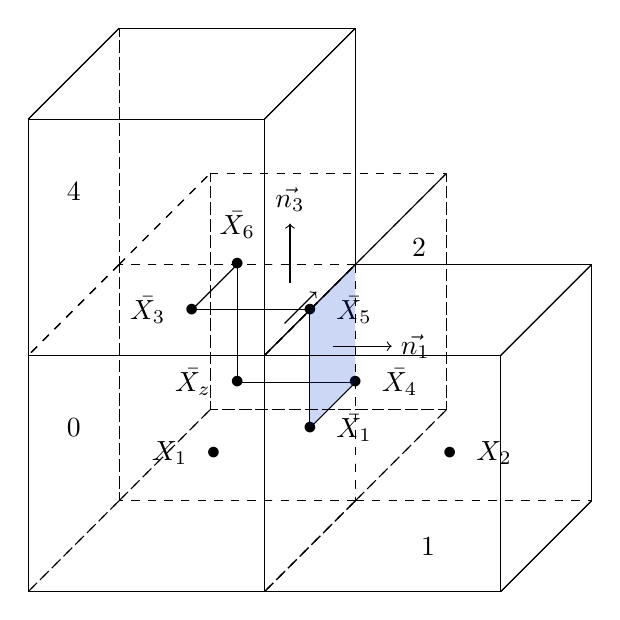
\begin{tikzpicture}[scale = 3, cm={1,0,-1,-1, (0,0)},y=-3.85mm, z = -1cm]

\node at (-1,-0.5,0.5) {$4$};
\node at (0,0.7,-0.2)  {$2$};
\node at (-1,-0.5,-0.5){$0$};
\node at (0.5,-0.5,-1) {$1$};
\node[label=left:$X_1$] at (-0.6,0,-0.8) {$\bullet$};
\node[label=right:$X_2$] at (0.4,0,-0.8)  {$\bullet$};
\node[label=left:$\bar{X_3}$] at (-0.5,-0.5,0)  {$\bullet$};
\node[label=above:$\bar{X_6}$] at (-0.5,0,0)  {$\bullet$};
\node[label=right:$\bar{X_5}$] at (0,-0.5,0)  {$\bullet$};
\node[label=left:$\bar{X_z}$] at (-0.5,0,-0.5)  {$\bullet$};
\node[label=right:$\bar{X_1}$] at (0,-0.5,-0.5)  {$\bullet$};
\node[label=right:$\bar{X_4}$] at (0,0,-0.5)  {$\bullet$};

%Area

\draw[] (-0.5,0,0)    -- (-0.5,-0.5,0);
\draw[] (-0.5,-0.5,0) -- (0,-0.5,0);
\draw[] (0,-0.5,0)    -- (0,-0.5,-0.5);
\draw[] (0,-0.5,-0.5) -- (0,0,-0.5);
\draw[] (0,0,-0.5)    -- (-0.5,0,-0.5);
\draw[] (-0.5,0,-0.5) -- (-0.5,0,0);

\definecolor{lila}{rgb}{0,0.2,0.8}
\begin{scope}
  \clip[postaction={fill=lila,fill opacity=0.2}](0,0,0) -- (0,-0.5,0) -- (0,-0.5,-0.5) -- (0,0,-0.5) -- (0,0,0);
\end{scope}

%Arrows
\draw[->] (-0.2,-0.2,0) -- (-0.2,-0.2,0.25);
\node at  (-0.2,-0.2,0.35) {$\vec{n_3}$};
\draw [->](0,-0.25,-0.25) -- (0.25,-0.25,-0.25);
\node at  (0.35,-0.25,-0.25) {$\vec{n_1}$};
\draw [->](-0.3,0,-0.25) -- (-0.3,0.35,-0.25);

%Cube Left Front Upper

%X-Y rectangle Z = 1
\draw[] (-1,-1,1) -- (0,-1,1);
\draw[] (0,-1,1)  -- (0,0,1);
\draw[] (0,0,1)   -- (-1,0,1);
\draw[] (-1,0,1)  -- (-1,-1,1);

%X-Z rectangle Y = -1
\draw[] (-1,-1,1) -- (-1,-1,0);
\draw[] (-1,-1,0) -- (0,-1,0);
\draw[] (0,-1,0)  -- (0,-1,1);
\draw[] (0,-1,1)  -- (-1,-1,1);

%Z-Y rectangle X = 0
\draw[] (0,-1,1) -- (0,-1,0);
\draw[] (0,-1,0) -- (0,0,0);
\draw[] (0,0,0)  -- (0,0,1);
\draw[]  (0,0,1) -- (0,-1,1);

%X-Y rectangle Z = 0
\draw[] (-1,-1,0) -- (0,-1,0);
\draw[dashed] (0,-1,0) -- (0,0,0);
\draw[dashed] (0,0,0)  -- (-1,0,0);
\draw[dashed] (-1,0,0) -- (-1,-1,0);

%Y-Z rectangle X = -1
\draw[] (-1,-1,0) -- (-1,-1,1);
\draw[] (-1,-1,1) -- (-1,0,1);
\draw[dashed] (-1,0,1) -- (-1,0,0);
\draw[dashed] (-1,0,0) -- (-1,-1,0);

%X-Z rectangle Y = 0
\draw[dashed] (0,0,0)  -- (-1,0,0);
\draw[dashed] (-1,0,0) -- (-1,0,1);
\draw[dashed] (0,0,0)  -- (0,0,1);
\draw[]       (0,0,1)  -- (-1,0,1);

%Cube Left Front Lower

%X-Y rectangle Z = -1
\draw[] (-1,-1,-1) -- (0,-1,-1);
\draw[dashed] (0,-1,-1)  -- (0,0,-1);
\draw[dashed] (0,0,-1)   -- (-1,0,-1);
\draw[dashed] (-1,0,-1)  -- (-1,-1,-1);

%X-Z rectangle Y = -1
\draw[] (-1,-1,-1) -- (-1,-1,0);
\draw[] (-1,-1,0) -- (0,-1,0);
\draw[] (0,-1,0)  -- (0,-1,-1);
\draw[] (0,-1,-1)  -- (-1,-1,-1);

%Z-Y rectangle X = 0
\draw[] (0,-1,-1) -- (0,-1,0);
\draw[dashed] (0,-1,0) -- (0,0,0);
\draw[dashed] (0,0,0)  -- (0,0,-1);
\draw[dashed]  (0,0,-1) -- (0,-1,-1);

%X-Y rectangle Z = 0
\draw[] (-1,-1,0) -- (0,-1,0);
\draw[dashed] (0,-1,0) -- (0,0,0);
\draw[dashed] (0,0,0)  -- (-1,0,0);
\draw[dashed] (-1,0,0) -- (-1,-1,0);

%Y-Z rectangle X = -1
\draw[] (-1,-1,0) -- (-1,-1,-1);
\draw[dashed] (-1,-1,-1) -- (-1,0,-1);
\draw[dashed] (-1,0,-1) -- (-1,0,0);
\draw[dashed] (-1,0,0) -- (-1,-1,0);

%X-Z rectangle Y = 0
\draw[dashed] (0,0,0)  -- (-1,0,0);
\draw[dashed] (-1,0,0) -- (-1,0,-1);
\draw[dashed] (0,0,0)  -- (0,0,-1);
\draw[dashed]       (0,0,-1)  -- (-1,0,-1);

%Cube Right Front Lower

%X-Y rectangle Z = -1
\draw[] (1,-1,-1) -- (0,-1,-1);
\draw[dashed] (0,-1,-1)  -- (0,0,-1);
\draw[dashed] (0,0,-1)   -- (1,0,-1);
\draw[] (1,0,-1)  -- (1,-1,-1);

%rX-Z rectangle Y = -1
\draw[] (1,-1,-1) -- (1,-1,0);
\draw[] (1,-1,0) -- (0,-1,0);
\draw[] (0,-1,0)  -- (0,-1,-1);
\draw[] (0,-1,-1)  -- (1,-1,-1);

%Y-Z rectangle X = 0
\draw[] (0,-1,-1) -- (0,-1,0);
\draw[] (0,-1,0) -- (0,0,0);
\draw[dashed] (0,0,0)  -- (0,0,-1);
\draw[dashed]  (0,0,-1) -- (0,-1,-1);

%X-Y rectangle Z = 0
\draw[] (1,-1,0) -- (0,-1,0);
\draw[dashed] (0,-1,0) -- (0,0,0);
\draw[dashed] (0,0,0)  -- (1,0,0);
\draw[] (1,0,0) -- (1,-1,0);

%Y-Z rectangle X = 1
\draw[] (1,-1,0) -- (1,-1,-1);
\draw[] (1,-1,-1) -- (1,0,-1);
\draw[] (1,0,-1) -- (1,0,0);
\draw[] (1,0,0) -- (1,-1,0);

%X-Z rectangle Y = 0
\draw[] (0,0,0)  -- (1,0,0);
\draw[] (1,0,0) -- (1,0,-1);
\draw[dashed] (0,0,0)  -- (0,0,-1);
\draw[dashed] (0,0,-1)  -- (1,0,-1);

%Cube Left Back Lower

%X-Y rectangle Z = -1
\draw[dashed] (-1,1,-1) -- (0,1,-1);
\draw[dashed] (0,1,-1)  -- (0,0,-1);
\draw[dashed] (0,0,-1)   -- (-1,0,-1);
\draw[dashed] (-1,0,-1)  -- (-1,1,-1);

%X-Z rectangle Y = 1
\draw[dashed] (-1,1,-1) -- (-1,1,0);
\draw[dashed] (-1,1,0) -- (0,1,0);
\draw[dashed] (0,1,0)  -- (0,1,-1);
\draw[dashed] (0,1,-1)  -- (-1,1,-1);

%Y-Z rectangle X = 0
\draw[dashed] (0,1,-1) -- (0,1,0);
\draw[] (0,1,0) -- (0,0,0);
\draw[dashed] (0,0,0)  -- (0,0,-1);
\draw[dashed]  (0,0,-1) -- (0,1,-1);

%X-Y rectangle Z = 0
\draw[dashed] (-1,1,0) -- (0,1,0);
\draw[dashed] (0,1,0) -- (0,0,0);
\draw[dashed] (0,0,0)  -- (-1,0,0);
\draw[dashed] (-1,0,0) -- (-1,1,0);

%Y-Z rectangle X = -1
\draw[dashed] (-1,1,0) -- (-1,1,-1);
\draw[dashed] (-1,1,-1) -- (-1,0,-1);
\draw[dashed] (-1,0,-1) -- (-1,0,0);
\draw[dashed] (-1,0,0) -- (-1,1,0);

%X-Z rectangle Y = 0
\draw[dashed] (0,0,0)  -- (-1,0,0);
\draw[dashed] (-1,0,0) -- (-1,0,-1);
\draw[dashed] (0,0,0)  -- (0,0,-1);
\draw[dashed]       (0,0,-1)  -- (-1,0,-1);







\end{tikzpicture}
\caption{case1.}
\end{figure}

\begin{figure}
\centering
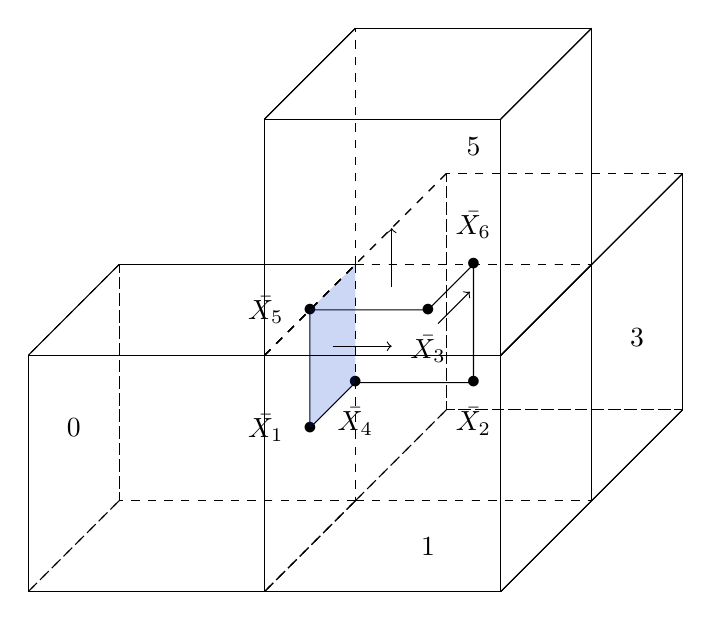
\begin{tikzpicture}[scale = 3, cm={1,0,-1,-1, (0,0)},y=-3.85mm, z = -1cm]

\node at (0.5,0,0.5)     {$5$};
\node at (1,0.5,-0.5)    {$3$};
\node at (0.5,-0.5,-1)   {$1$};
\node at (-1,-0.5,-0.5)  {$0$};

\node[label=left:$\bar{X_1}$] at (0,-0.5,-0.5) {$\bullet$};
\node[label=left:$\bar{X_5}$] at (0,-0.5,0) {$\bullet$};
\node[label=below:$\bar{X_3}$] at (0.5,-0.5,0) {$\bullet$};
\node[label=below:$\bar{X_4}$] at (0,0,-0.5) {$\bullet$};
\node[label=below:$\bar{X_2}$] at (0.5,0,-0.5) {$\bullet$};
\node[label=above:$\bar{X_6}$] at (0.5,0,0) {$\bullet$};

%Area
\draw [] (0,-0.5,0) -- (0,-0.5,-0.5) -- (0,0,-0.5) -- (0.5,0,-0.5) -- (0.5,0,0) -- (0.5,-0.5,0) -- (0,-0.5,0);

\definecolor{lila}{rgb}{0,0.2,0.8}
\begin{scope}
  \clip[postaction={fill=lila,fill opacity=0.2}](0,0,0) -- (0,-0.5,0) -- (0,-0.5,-0.5) -- (0,0,-0.5) -- (0,0,0);
\end{scope}

%Arrows
\draw[->] (0.25,-0.25,0) -- (0.25,-0.25,0.25);
\draw[->] (0.35,0,-0.25) -- (0.35,0.35,-0.25);
\draw[->] (0,-0.25,-0.25) -- (0.25,-0.25,-0.25);

%Cube Left Front Lower

%X-Y rectangle Z = -1
\draw[] (-1,-1,-1) -- (0,-1,-1);
\draw[dashed] (0,-1,-1)  -- (0,0,-1);
\draw[dashed] (0,0,-1)   -- (-1,0,-1);
\draw[dashed] (-1,0,-1)  -- (-1,-1,-1);

%X-Z rectangle Y = -1
\draw[] (-1,-1,-1) -- (-1,-1,0);
\draw[] (-1,-1,0) -- (0,-1,0);
\draw[] (0,-1,0)  -- (0,-1,-1);
\draw[] (0,-1,-1)  -- (-1,-1,-1);

%Z-Y rectangle X = 0
\draw[] (0,-1,-1) -- (0,-1,0);
\draw[dashed] (0,-1,0) -- (0,0,0);
\draw[dashed] (0,0,0)  -- (0,0,-1);
\draw[dashed]  (0,0,-1) -- (0,-1,-1);

%X-Y rectangle Z = 0
\draw[] (-1,-1,0) -- (0,-1,0);
\draw[dashed] (0,-1,0) -- (0,0,0);
\draw[] (0,0,0)  -- (-1,0,0);
\draw[] (-1,0,0) -- (-1,-1,0);

%Y-Z rectangle X = -1
\draw[] (-1,-1,0) -- (-1,-1,-1);
\draw[dashed] (-1,-1,-1) -- (-1,0,-1);
\draw[dashed] (-1,0,-1) -- (-1,0,0);
\draw[dashed] (-1,0,0) -- (-1,-1,0);

%X-Z rectangle Y = 0
\draw[dashed] (0,0,0)  -- (-1,0,0);
\draw[dashed] (-1,0,0) -- (-1,0,-1);
\draw[dashed] (0,0,0)  -- (0,0,-1);
\draw[dashed]       (0,0,-1)  -- (-1,0,-1);

%Cube Right Front Upper

%X-Y rectangle Z = 1
\draw[] (1,-1,1) -- (0,-1,1);
\draw[] (0,-1,1)  -- (0,0,1);
\draw[] (0,0,1)   -- (1,0,1);
\draw[] (1,0,1)  -- (1,-1,1);

%rX-Z rectangle Y = -1
\draw[] (1,-1,1) -- (1,-1,0);
\draw[] (1,-1,0) -- (0,-1,0);
\draw[] (0,-1,0)  -- (0,-1,1);
\draw[] (0,-1,1)  -- (1,-1,1);

%Y-Z rectangle X = 0
\draw[] (0,-1,1) -- (0,-1,0);
\draw[dashed] (0,-1,0) -- (0,0,0);
\draw[dashed] (0,0,0)  -- (0,0,1);
\draw[]  (0,0,1) -- (0,-1,1);

%X-Y rectangle Z = 0
\draw[] (1,-1,0) -- (0,-1,0);
\draw[dashed] (0,-1,0) -- (0,0,0);
\draw[dashed] (0,0,0)  -- (1,0,0);
\draw[] (1,0,0) -- (1,-1,0);

%Y-Z rectangle X = 1
\draw[] (1,-1,0) -- (1,-1,1);
\draw[] (1,-1,1) -- (1,0,1);
\draw[] (1,0,1) -- (1,0,0);
\draw[] (1,0,0) -- (1,-1,0);

%X-Z rectangle Y = 0
\draw[dashed] (0,0,0)  -- (1,0,0);
\draw[] (1,0,0) -- (1,0,1);
\draw[dashed] (0,0,0)  -- (0,0,1);
\draw[]       (0,0,1)  -- (1,0,1);

%Cube Right Front Lower

%X-Y rectangle Z = -1
\draw[] (1,-1,-1) -- (0,-1,-1);
\draw[dashed] (0,-1,-1)  -- (0,0,-1);
\draw[dashed] (0,0,-1)   -- (1,0,-1);
\draw[] (1,0,-1)  -- (1,-1,-1);

%rX-Z rectangle Y = -1
\draw[] (1,-1,-1) -- (1,-1,0);
\draw[] (1,-1,0) -- (0,-1,0);
\draw[] (0,-1,0)  -- (0,-1,-1);
\draw[] (0,-1,-1)  -- (1,-1,-1);

%Y-Z rectangle X = 0
\draw[] (0,-1,-1) -- (0,-1,0);
\draw[dashed] (0,-1,0) -- (0,0,0);
\draw[dashed] (0,0,0)  -- (0,0,-1);
\draw[dashed]  (0,0,-1) -- (0,-1,-1);

%X-Y rectangle Z = 0
\draw[] (1,-1,0) -- (0,-1,0);
\draw[dashed] (0,-1,0) -- (0,0,0);
\draw[dashed] (0,0,0)  -- (1,0,0);
\draw[] (1,0,0) -- (1,-1,0);

%Y-Z rectangle X = 1
\draw[] (1,-1,0) -- (1,-1,-1);
\draw[] (1,-1,-1) -- (1,0,-1);
\draw[] (1,0,-1) -- (1,0,0);
\draw[] (1,0,0) -- (1,-1,0);

%X-Z rectangle Y = 0
\draw[dashed] (0,0,0)  -- (1,0,0);
\draw[] (1,0,0) -- (1,0,-1);
\draw[dashed] (0,0,0)  -- (0,0,-1);
\draw[dashed] (0,0,-1)  -- (1,0,-1);

%Cube Right Back Lower

%X-Y rectangle Z = -1
\draw[dashed] (1,1,-1) -- (0,1,-1);
\draw[dashed] (0,1,-1)  -- (0,0,-1);
\draw[dashed] (0,0,-1)   -- (1,0,-1);
\draw[] (1,0,-1)  -- (1,1,-1);

%X-Z rectangle Y = 1
\draw[] (1,1,-1) -- (1,1,0);
\draw[dashed] (1,1,0) -- (0,1,0);
\draw[dashed] (0,1,0)  -- (0,1,-1);
\draw[dashed] (0,1,-1)  -- (1,1,-1);

%Y-Z rectangle X = 0
\draw[dashed] (0,1,-1) -- (0,1,0);
\draw[dashed] (0,1,0) -- (0,0,0);
\draw[dashed] (0,0,0)  -- (0,0,-1);
\draw[dashed]  (0,0,-1) -- (0,1,-1);

%X-Y rectangle Z = 0
\draw[dashed] (1,1,0) -- (0,1,0);
\draw[dashed] (0,1,0) -- (0,0,0);
\draw[dashed] (0,0,0)  -- (1,0,0);
\draw[] (1,0,0) -- (1,1,0);

%Y-Z rectangle X = 1
\draw[] (1,1,0) -- (1,1,-1);
\draw[] (1,1,-1) -- (1,0,-1);
\draw[] (1,0,-1) -- (1,0,0);
\draw[] (1,0,0) -- (1,1,0);

%X-Z rectangle Y = 0
\draw[dashed] (0,0,0)  -- (1,0,0);
\draw[] (1,0,0) -- (1,0,-1);
\draw[dashed] (0,0,0)  -- (0,0,-1);
\draw[dashed]       (0,0,-1)  -- (1,0,-1);







\end{tikzpicture}
\caption{case2.}
\end{figure}

\begin{figure}
\centering
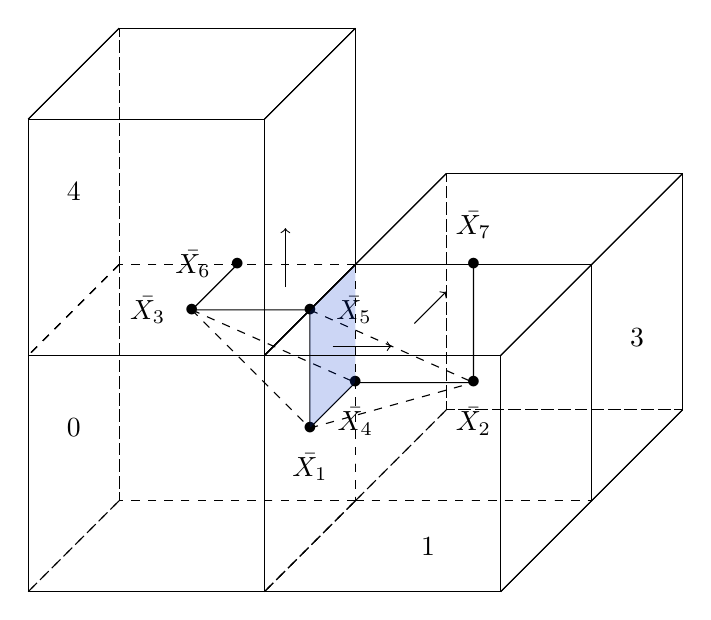
\begin{tikzpicture}[scale = 3, cm={1,0,-1,-1, (0,0)},y=-3.85mm, z = -1cm]

\node at (0.5,-0.5,-1)  {$1$};
\node at (1,0.5,-0.5)      {$3$};
\node at (-1,-0.5,0.5)  {$4$};
\node at (-1,-0.5,-0.5) {$0$};

\node[label=below:$\bar{X_1}$] at (0,-0.5,-0.5) {$\bullet$};
\node[label=below:$\bar{X_2}$] at (0.5,0,-0.5) {$\bullet$};
\node[label=below:$\bar{X_4}$] at (0,0,-0.5) {$\bullet$};
\node[label=right:$\bar{X_5}$] at (0,-0.5,0) {$\bullet$};
\node[label=left:$\bar{X_3}$] at (-0.5,-0.5,0) {$\bullet$};
\node[label=left:$\bar{X_6}$] at (-0.5,0,0) {$\bullet$};
\node[label=above:$\bar{X_7}$] at (0.5,0,0) {$\bullet$};

%Area
\draw[] (-0.5,0,0)--(-0.5,-0.5,0)--(0,-0.5,0)--(0,-0.5,-0.5)--(0,0,-0.5)--(0.5,0,-0.5)--(0.5,0,0);
\draw[dashed] (0,-0.5,-0.5)--(0.5,0,-0.5);
\draw[dashed] (-0.5,-0.5,0)--(0,-0.5,-0.5);
\draw[dashed] (-0.5,-0.5,0)--(0,0,-0.5);
\draw[dashed] (0,-0.5,0)   --(0.5,0,-0.5);

\definecolor{lila}{rgb}{0,0.2,0.8}
\begin{scope}
  \clip[postaction={fill=lila,fill opacity=0.2}](0,0,0) -- (0,-0.5,0) -- (0,-0.5,-0.5) -- (0,0,-0.5) -- (0,0,0);
\end{scope}

%Arrows
\draw[->] (0,-0.25,-0.25) -- (0.25,-0.25,-0.25);
\draw[->] (0.25,0,-0.25)  -- (0.25,0.35,-0.25);
\draw[->] (-0.2,-0.25,0)  -- (-0.2,-0.25,0.25);

%Cube Left Front Lower

%X-Y rectangle Z = -1
\draw[] (-1,-1,-1) -- (0,-1,-1);
\draw[dashed] (0,-1,-1)  -- (0,0,-1);
\draw[dashed] (0,0,-1)   -- (-1,0,-1);
\draw[dashed] (-1,0,-1)  -- (-1,-1,-1);

%X-Z rectangle Y = -1
\draw[] (-1,-1,-1) -- (-1,-1,0);
\draw[] (-1,-1,0) -- (0,-1,0);
\draw[] (0,-1,0)  -- (0,-1,-1);
\draw[] (0,-1,-1)  -- (-1,-1,-1);

%Z-Y rectangle X = 0
\draw[] (0,-1,-1) -- (0,-1,0);
\draw[] (0,-1,0) -- (0,0,0);
\draw[dashed] (0,0,0)  -- (0,0,-1);
\draw[dashed]  (0,0,-1) -- (0,-1,-1);

%X-Y rectangle Z = 0
\draw[] (-1,-1,0) -- (0,-1,0);
\draw[] (0,-1,0) -- (0,0,0);
\draw[dashed] (0,0,0)  -- (-1,0,0);
\draw[dashed] (-1,0,0) -- (-1,-1,0);

%Y-Z rectangle X = -1
\draw[] (-1,-1,0) -- (-1,-1,-1);
\draw[dashed] (-1,-1,-1) -- (-1,0,-1);
\draw[dashed] (-1,0,-1) -- (-1,0,0);
\draw[dashed] (-1,0,0) -- (-1,-1,0);

%X-Z rectangle Y = 0
\draw[dashed] (0,0,0)  -- (-1,0,0);
\draw[dashed] (-1,0,0) -- (-1,0,-1);
\draw[dashed] (0,0,0)  -- (0,0,-1);
\draw[dashed]       (0,0,-1)  -- (-1,0,-1);

%Cube Right Front Lower

%X-Y rectangle Z = -1
\draw[] (1,-1,-1) -- (0,-1,-1);
\draw[dashed] (0,-1,-1)  -- (0,0,-1);
\draw[dashed] (0,0,-1)   -- (1,0,-1);
\draw[] (1,0,-1)  -- (1,-1,-1);

%rX-Z rectangle Y = -1
\draw[] (1,-1,-1) -- (1,-1,0);
\draw[] (1,-1,0) -- (0,-1,0);
\draw[] (0,-1,0)  -- (0,-1,-1);
\draw[] (0,-1,-1)  -- (1,-1,-1);

%Y-Z rectangle X = 0
\draw[] (0,-1,-1) -- (0,-1,0);
\draw[] (0,-1,0) -- (0,0,0);
\draw[dashed] (0,0,0)  -- (0,0,-1);
\draw[dashed]  (0,0,-1) -- (0,-1,-1);

%X-Y rectangle Z = 0
\draw[] (1,-1,0) -- (0,-1,0);
\draw[] (0,-1,0) -- (0,0,0);
\draw[] (0,0,0)  -- (1,0,0);
\draw[] (1,0,0) -- (1,-1,0);

%Y-Z rectangle X = 1
\draw[] (1,-1,0) -- (1,-1,-1);
\draw[] (1,-1,-1) -- (1,0,-1);
\draw[] (1,0,-1) -- (1,0,0);
\draw[] (1,0,0) -- (1,-1,0);

%X-Z rectangle Y = 0
\draw[] (0,0,0)  -- (1,0,0);
\draw[] (1,0,0) -- (1,0,-1);
\draw[dashed] (0,0,0)  -- (0,0,-1);
\draw[dashed] (0,0,-1)  -- (1,0,-1);

%Cube Right Back Lower

%X-Y rectangle Z = -1
\draw[dashed] (1,1,-1) -- (0,1,-1);
\draw[dashed] (0,1,-1)  -- (0,0,-1);
\draw[dashed] (0,0,-1)   -- (1,0,-1);
\draw[] (1,0,-1)  -- (1,1,-1);

%X-Z rectangle Y = 1
\draw[] (1,1,-1) -- (1,1,0);
\draw[] (1,1,0) -- (0,1,0);
\draw[dashed] (0,1,0)  -- (0,1,-1);
\draw[dashed] (0,1,-1)  -- (1,1,-1);

%Y-Z rectangle X = 0
\draw[dashed] (0,1,-1) -- (0,1,0);
\draw[] (0,1,0) -- (0,0,0);
\draw[dashed] (0,0,0)  -- (0,0,-1);
\draw[dashed]  (0,0,-1) -- (0,1,-1);

%X-Y rectangle Z = 0
\draw[] (1,1,0) -- (0,1,0);
\draw[] (0,1,0) -- (0,0,0);
\draw[] (0,0,0)  -- (1,0,0);
\draw[] (1,0,0) -- (1,1,0);

%Y-Z rectangle X = 1
\draw[] (1,1,0) -- (1,1,-1);
\draw[] (1,1,-1) -- (1,0,-1);
\draw[] (1,0,-1) -- (1,0,0);
\draw[] (1,0,0) -- (1,1,0);

%X-Z rectangle Y = 0
\draw[] (0,0,0)  -- (1,0,0);
\draw[] (1,0,0) -- (1,0,-1);
\draw[dashed] (0,0,0)  -- (0,0,-1);
\draw[dashed]       (0,0,-1)  -- (1,0,-1);

%Cube Left Front Upper

%X-Y rectangle Z = 1
\draw[] (-1,-1,1) -- (0,-1,1);
\draw[] (0,-1,1)  -- (0,0,1);
\draw[] (0,0,1)   -- (-1,0,1);
\draw[] (-1,0,1)  -- (-1,-1,1);

%X-Z rectangle Y = -1
\draw[] (-1,-1,1) -- (-1,-1,0);
\draw[] (-1,-1,0) -- (0,-1,0);
\draw[] (0,-1,0)  -- (0,-1,1);
\draw[] (0,-1,1)  -- (-1,-1,1);

%Z-Y rectangle X = 0
\draw[] (0,-1,1) -- (0,-1,0);
\draw[] (0,-1,0) -- (0,0,0);
\draw[] (0,0,0)  -- (0,0,1);
\draw[]  (0,0,1) -- (0,-1,1);

%X-Y rectangle Z = 0
\draw[] (-1,-1,0) -- (0,-1,0);
\draw[] (0,-1,0) -- (0,0,0);
\draw[dashed] (0,0,0)  -- (-1,0,0);
\draw[dashed] (-1,0,0) -- (-1,-1,0);

%Y-Z rectangle X = -1
\draw[] (-1,-1,0) -- (-1,-1,1);
\draw[] (-1,-1,1) -- (-1,0,1);
\draw[dashed] (-1,0,1) -- (-1,0,0);
\draw[dashed] (-1,0,0) -- (-1,-1,0);

%X-Z rectangle Y = 0
\draw[dashed] (0,0,0)  -- (-1,0,0);
\draw[dashed] (-1,0,0) -- (-1,0,1);
\draw[] (0,0,0)  -- (0,0,1);
\draw[]       (0,0,1)  -- (-1,0,1);

\end{tikzpicture}
\caption{case3.}
\end{figure}

\begin{figure}
\centering
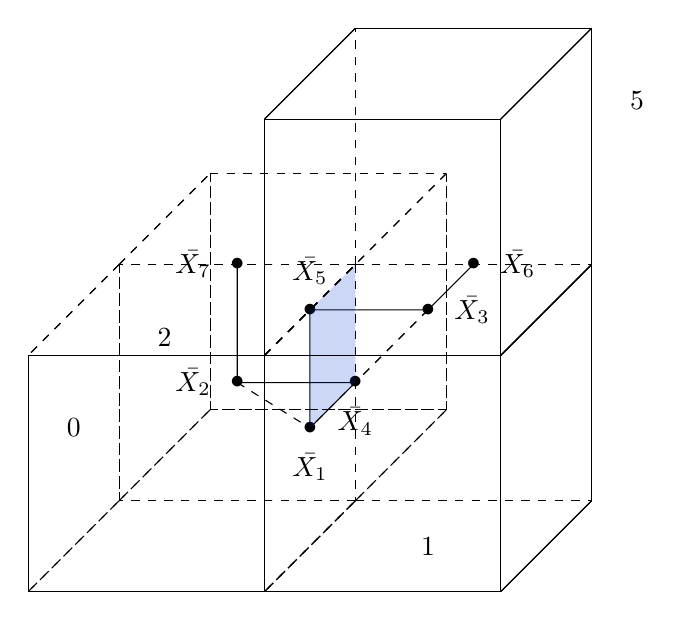
\begin{tikzpicture}[scale = 3, cm={1,0,-1,-1, (0,0)},y=-3.85mm, z = -1cm]

\node at (0.5,-0.5,-1) {$1$};
\node at (-1,0.5,-0.5) {$2$};
\node at (1,0.5,0.5)   {$5$};
\node at (-1,-0.5,-0.5){$0$};

\node[label=below:$\bar{X_1}$] at (0,-0.5,-0.5) {$\bullet$};
\node[label=below:$\bar{X_4}$] at (0,0,-0.5) {$\bullet$};
\node[label=above:$\bar{X_5}$] at (0,-0.5,0) {$\bullet$};
\node[label=left:$\bar{X_2}$] at  (-0.5,0,-0.5) {$\bullet$};
\node[label=left:$\bar{X_7}$] at (-0.5,0,0) {$\bullet$};
\node[label=right:$\bar{X_3}$] at (0.5,-0.5,0) {$\bullet$};
\node[label=right:$\bar{X_6}$] at (0.5,0,0) {$\bullet$};

%Area

\draw (-0.5,0,0)--(-0.5,0,-0.5)--(0,0,-0.5)--(0,-0.5,-0.5)--(0,-0.5,0)--(0.5,-0.5,0)--(0.5,0,0);
\draw[dashed] (-0.5,0,-0.5)--(0,-0.5,-0.5);
\draw[dashed] (-0.5,0,-0.5)--(0,0,-0.5);
\draw[dashed] (0.5,-0.5,0)-- (0,-0.5,-0.5);
\draw[dashed] (0.5,-0.5,0)-- (0,0,-0.5);

\definecolor{lila}{rgb}{0,0.2,0.8}
\begin{scope}
  \clip[postaction={fill=lila,fill opacity=0.2}](0,0,0) -- (0,-0.5,0) -- (0,-0.5,-0.5) -- (0,0,-0.5) -- (0,0,0);
\end{scope}


%Cube Left Front Lower

%X-Y rectangle Z = -1
\draw[] (-1,-1,-1) -- (0,-1,-1);
\draw[dashed] (0,-1,-1)  -- (0,0,-1);
\draw[dashed] (0,0,-1)   -- (-1,0,-1);
\draw[dashed] (-1,0,-1)  -- (-1,-1,-1);

%X-Z rectangle Y = -1
\draw[] (-1,-1,-1) -- (-1,-1,0);
\draw[] (-1,-1,0) -- (0,-1,0);
\draw[] (0,-1,0)  -- (0,-1,-1);
\draw[] (0,-1,-1)  -- (-1,-1,-1);

%Z-Y rectangle X = 0
\draw[] (0,-1,-1) -- (0,-1,0);
\draw[dashed] (0,-1,0) -- (0,0,0);
\draw[dashed] (0,0,0)  -- (0,0,-1);
\draw[dashed]  (0,0,-1) -- (0,-1,-1);

%X-Y rectangle Z = 0
\draw[] (-1,-1,0) -- (0,-1,0);
\draw[dashed] (0,-1,0) -- (0,0,0);
\draw[dashed] (0,0,0)  -- (-1,0,0);
\draw[dashed] (-1,0,0) -- (-1,-1,0);

%Y-Z rectangle X = -1
\draw[] (-1,-1,0) -- (-1,-1,-1);
\draw[dashed] (-1,-1,-1) -- (-1,0,-1);
\draw[dashed] (-1,0,-1) -- (-1,0,0);
\draw[dashed] (-1,0,0) -- (-1,-1,0);

%X-Z rectangle Y = 0
\draw[dashed] (0,0,0)  -- (-1,0,0);
\draw[dashed] (-1,0,0) -- (-1,0,-1);
\draw[dashed] (0,0,0)  -- (0,0,-1);
\draw[dashed]       (0,0,-1)  -- (-1,0,-1);

%Cube Right Front Upper

%X-Y rectangle Z = 1
\draw[] (1,-1,1) -- (0,-1,1);
\draw[] (0,-1,1)  -- (0,0,1);
\draw[] (0,0,1)   -- (1,0,1);
\draw[] (1,0,1)  -- (1,-1,1);

%rX-Z rectangle Y = -1
\draw[] (1,-1,1) -- (1,-1,0);
\draw[] (1,-1,0) -- (0,-1,0);
\draw[] (0,-1,0)  -- (0,-1,1);
\draw[] (0,-1,1)  -- (1,-1,1);

%Y-Z rectangle X = 0
\draw[] (0,-1,1) -- (0,-1,0);
\draw[dashed] (0,-1,0) -- (0,0,0);
\draw[dashed] (0,0,0)  -- (0,0,1);
\draw[]  (0,0,1) -- (0,-1,1);

%X-Y rectangle Z = 0
\draw[] (1,-1,0) -- (0,-1,0);
\draw[dashed] (0,-1,0) -- (0,0,0);
\draw[dashed] (0,0,0)  -- (1,0,0);
\draw[] (1,0,0) -- (1,-1,0);

%Y-Z rectangle X = 1
\draw[] (1,-1,0) -- (1,-1,1);
\draw[] (1,-1,1) -- (1,0,1);
\draw[] (1,0,1) -- (1,0,0);
\draw[] (1,0,0) -- (1,-1,0);

%X-Z rectangle Y = 0
\draw[dashed] (0,0,0)  -- (1,0,0);
\draw[] (1,0,0) -- (1,0,1);
\draw[dashed] (0,0,0)  -- (0,0,1);
\draw[]       (0,0,1)  -- (1,0,1);

%Cube Right Front Lower

%X-Y rectangle Z = -1
\draw[] (1,-1,-1) -- (0,-1,-1);
\draw[dashed] (0,-1,-1)  -- (0,0,-1);
\draw[dashed] (0,0,-1)   -- (1,0,-1);
\draw[] (1,0,-1)  -- (1,-1,-1);

%rX-Z rectangle Y = -1
\draw[] (1,-1,-1) -- (1,-1,0);
\draw[] (1,-1,0) -- (0,-1,0);
\draw[] (0,-1,0)  -- (0,-1,-1);
\draw[] (0,-1,-1)  -- (1,-1,-1);

%Y-Z rectangle X = 0
\draw[] (0,-1,-1) -- (0,-1,0);
\draw[dashed] (0,-1,0) -- (0,0,0);
\draw[dashed] (0,0,0)  -- (0,0,-1);
\draw[dashed]  (0,0,-1) -- (0,-1,-1);

%X-Y rectangle Z = 0
\draw[] (1,-1,0) -- (0,-1,0);
\draw[dashed] (0,-1,0) -- (0,0,0);
\draw[dashed] (0,0,0)  -- (1,0,0);
\draw[] (1,0,0) -- (1,-1,0);

%Y-Z rectangle X = 1
\draw[] (1,-1,0) -- (1,-1,-1);
\draw[] (1,-1,-1) -- (1,0,-1);
\draw[] (1,0,-1) -- (1,0,0);
\draw[] (1,0,0) -- (1,-1,0);

%X-Z rectangle Y = 0
\draw[dashed] (0,0,0)  -- (1,0,0);
\draw[] (1,0,0) -- (1,0,-1);
\draw[dashed] (0,0,0)  -- (0,0,-1);
\draw[dashed] (0,0,-1)  -- (1,0,-1);

%Cube Left Back Lower

%X-Y rectangle Z = -1
\draw[dashed] (-1,1,-1) -- (0,1,-1);
\draw[dashed] (0,1,-1)  -- (0,0,-1);
\draw[dashed] (0,0,-1)   -- (-1,0,-1);
\draw[dashed] (-1,0,-1)  -- (-1,1,-1);

%X-Z rectangle Y = 1
\draw[dashed] (-1,1,-1) -- (-1,1,0);
\draw[dashed] (-1,1,0) -- (0,1,0);
\draw[dashed] (0,1,0)  -- (0,1,-1);
\draw[dashed] (0,1,-1)  -- (-1,1,-1);

%Y-Z rectangle X = 0
\draw[dashed] (0,1,-1) -- (0,1,0);
\draw[dashed] (0,1,0) -- (0,0,0);
\draw[dashed] (0,0,0)  -- (0,0,-1);
\draw[dashed]  (0,0,-1) -- (0,1,-1);

%X-Y rectangle Z = 0
\draw[dashed] (-1,1,0) -- (0,1,0);
\draw[dashed] (0,1,0) -- (0,0,0);
\draw[dashed] (0,0,0)  -- (-1,0,0);
\draw[dashed] (-1,0,0) -- (-1,1,0);

%Y-Z rectangle X = -1
\draw[dashed] (-1,1,0) -- (-1,1,-1);
\draw[dashed] (-1,1,-1) -- (-1,0,-1);
\draw[dashed] (-1,0,-1) -- (-1,0,0);
\draw[dashed] (-1,0,0) -- (-1,1,0);

%X-Z rectangle Y = 0
\draw[dashed] (0,0,0)  -- (-1,0,0);
\draw[dashed] (-1,0,0) -- (-1,0,-1);
\draw[dashed] (0,0,0)  -- (0,0,-1);
\draw[dashed]       (0,0,-1)  -- (-1,0,-1);

\end{tikzpicture}
\caption{case4.}
\end{figure}

\end{document}
